\documentclass[11pt]{article}
\usepackage[margin=0.5in]{geometry}
\usepackage{todonotes}
\usepackage{natbib}
\usepackage{graphicx}
\usepackage{listings}
\usepackage{color}
\usepackage{hyperref}
\usepackage{multirow}
\usepackage{pifont}
\usepackage{xcolor,colortbl}
\usepackage{hyperref}
\hypersetup{colorlinks=true,linkcolor=black,citecolor=blue,filecolor=black,urlcolor=blue}
\usepackage{amsmath}
\usepackage{xspace}
\usepackage{makecell}
\usepackage{ulem} % provides sout
\usepackage{minted} % Provides listing environment


\newcommand{\tristan}[1]{\color{orange}\textbf{From Tristan:} #1\color{black}\xspace}
\newcommand{\tristanmod}[2]{\color{orange}\sout{#1} #2\color{black}\xspace}

\newcommand{\Yohan}[1]{\color{green!75!black}\textbf{Yohan:} #1\color{black}\xspace}
\newcommand{\cross}[0]{\cellcolor{red!65}\ding{53}}
\newcommand{\valid}[0]{\cellcolor{green!75!black}\ding{51}}
\newcommand{\warn}[0]{\cellcolor{orange!75}?}
\newcommand{\pytracer}[0]{PyTracer\xspace}

\usepackage{tabularx} % provides tabularx to adjust table column sizes to page size
% define thickline for use in tables
\makeatletter
\newcommand{\thickhline}{%
    \noalign {\ifnum 0=`}\fi \hrule height 1pt
    \futurelet \reserved@a \@xhline
}
\newcolumntype{"}{@{\hskip\tabcolsep\vrule width 1pt\hskip\tabcolsep}}
\makeatother


\lstdefinestyle{customPython}{
  belowcaptionskip=1\baselineskip,
  breaklines=true,
  xleftmargin=\parindent,
  language=Python,
  showstringspaces=false,
  basicstyle=\scriptsize\ttfamily,
  keywordstyle=\bfseries\color[rgb]{0.580, 0.000, 0.827},
  %{purple!40!lightgray},
  commentstyle=\itshape\color{green!40!black},
  identifierstyle=\bfseries\color{cyan!75!black},
  stringstyle=\color{orange},
  deletekeywords={double,float},
  classoffset=1, % starting new class
  otherkeywords={double,float},
  morekeywords={double,float},
  keywordstyle=\bfseries\color{green!55!black},
  classoffset=0
}

\lstdefinestyle{customC}{
  belowcaptionskip=1\baselineskip,
  breaklines=true,
  xleftmargin=\parindent,
  language=C,
  showstringspaces=false,
  basicstyle=\scriptsize\ttfamily,
  keywordstyle=\bfseries\color[rgb]{0.580, 0.000, 0.827},
  %{purple!40!lightgray},
  commentstyle=\itshape\color{green!40!black},
  identifierstyle=\bfseries\color{cyan!75!black},
  stringstyle=\color{orange},
  deletekeywords={double,float},
  classoffset=1, % starting new class
  otherkeywords={double,float},
  morekeywords={double,float},
  keywordstyle=\bfseries\color{green!55!black},
  classoffset=0
}


\begin{document}

\makeatletter
\let\orig@lstnumber=\thelstnumber
\newcommand\lstsetnumber[1]{\gdef\thelstnumber{#1}}
\newcommand\lstresetnumber{\global\let\thelstnumber=\orig@lstnumber}
\makeatother

\title{PyTracer: Automatically profiling numerical instabilities in Python}
\author{Yohan Chatelain$^1$, Gregory Kiar$^2$, Nigel Young$^1$, Tristan Glatard$^1$\\
$^1$Department of Computer Science and Software Engineering, Concordia University, Montreal, Canada\\
$^2$Center for the Developing Brain, Child Mind Institute, New York, NY, USA}
\date{}
\maketitle

\begin{abstract}
[abstract goes here]
\end{abstract}

\section{Introduction}

The scientific Python ecosystem is a central component of scientific
analyses due to its rich data manipulation, array programming,
numerical analysis, and visualization tools. In particular, libraries such
as NumPy~\cite{harris2020array}, SciPy~\cite{virtanen2020scipy}, scikit-learn~\cite{pedregosa2011scikit} or PyTorch~\cite{paszke2019pytorch} are used in hundreds of publications every year, providing a reference set of high-quality open-source core scientific libraries. Diverse research groups built numerous domain-specific data analysis pipelines from this ecosystem, leveraging Python's simplicity and expressivity. 

Numerical stability is a crucial requirement of reliable scientific data
processing. In unstable analyses, small numerical perturbations introduced by data noise, software and hardware updates, or parallelization lead to substantial deviations in final results and potentially different scientific conclusions, threatening the reliability of computational analyses. Numerical stability analyses need to be conducted systematically to address this issue. However, no practical tool currently exists to conduct such analyses on Python programs.

We present PyTracer, a numerical stability analyzer for Python programs.
PyTracer adopts a dynamic approach that evaluates numerical stability using program execution traces, enabling scaling to large programs without manual intervention. In contrast, theoretical approaches based on condition number or backward error analyses require detailed modeling of the program and its numerical implementation. Similarly, static code analysis techniques such as Frama-C~\cite{cuoq2012frama}, Gappa~\cite{de2010certifying} or Flocq~\cite{boldo2011flocq} hardly scale to large codebases, particularly in dynamically-typed languages such as Python.

PyTracer estimates the significant digits of Python floating-point variables by combining program traces obtained with different numerical perturbations, which requires (1) tracing floating-point computations along program executions, (2) generating numerically-perturbed executions, and (3) visualizing stability evaluations. PyTracer addresses these requirements with:
Dynamic instrumentation of Python functions, modules, and classes through meta-programming
A ``fuzzy" Python interpreter instrumented with Monte-Carlo arithmetic
An interactive Plotly dashboard to visualize stability measures throughout program executions

Through stability evaluations of 
SciPy, scikit-learn, and pyAFQ~\cite{kruper2021evaluating} --- an analysis toolbox for diffusion magnetic resonance imaging --- we demonstrate PyTracer as a practical solution to review the numerical stability of extensive code bases. The remainder of this manuscript describes related approaches, presents the design of PyTracer, and demonstrates its potential in various use cases.


\section{Related work}

Several tools have been and continue to be developed to assess numerical quality. Those tools can be divided into two main categories depending on whether they adopt a static or a dynamic approach.
The static analysis produces theoretically valid error bounds, while dynamic analysis is generally more scalable, although it only provides experimental estimations.
\pytracer adopts the dynamic approach due to its scalability to large existing code bases. Dynamic approaches typically rely on the tracing of floating-point computations to detect instabilities and visualize them. The remainder of this section reviews existing approaches for each of these three steps. 

% In this section, we review tools and theoretical frameworks related to \pytracer components.
% We start by reviewing state-of-the-art dynamic tools for detecting numerical instabilities.
% Then, we focus on existing theoretical approaches for perturbations-based techniques to detect numerical instabilities,
% \pytracer being agnostic to perturbation technique used. Finally, we review visualization tools 
% aiming at detecting numerical instabilities over execution time.

\label{sec:soa}
\subsection{Numerical tracing techniques}
Tools to trace floating-point computations for C, C++, or FORTRAN programs are plethora due to the prevalence of these languages in High-Performance Computing (HPC). 
The main tracing techniques are source-to-source, compiler-based transformations, and dynamic binary instrumentation.

The Source-to-source technique requires a rewriting of the application to use modify floating-point types.
CADNA~\cite{jezequel2008cadna} is a library for C, C++ and Fortran  implementing the CESTAC~\cite{vignes1993stochastic} stochastic arithmetic.
pLiner uses source-to-source transformation at the Abstract Syntax Tree (AST)  level to rewrite parts of code with higher precision. 
Shaman~\cite{demeure_phd} is a C++ library that uses a first-order error model to propagate numerical error. 
MCAlib~\cite{frechtling2015mcalib} is a C library that implements the Monte Carlo Arithmetic (MCA)~\cite{parker1997monte} using the MPFR~\cite{fousse2007mpfr} library.
The work in~\cite{tang2016software} proposed a source-to-source framework for executing targeted code in infinite and fixed precision with and without using stochastic arithmetic.

The compiler-based approach uses a compiler to analyze or replace floating-point expressions with other models automatically. 
Verificarlo~\cite{verificarlo} is a compiler that supports different types of arithmetic instrumentations, including MCA. 
The work in ~\cite{bao2013fly} modified the GNU Compiler Collection (GCC) to track local floating-point errors across executions. pLiner~\cite{guo2020pliner} is a root cause analyzer based on the Clang compiler that detects floating-point operations responsible for result variability. 
PFPSanitizer~\cite{chowdhary2020debugging,chowdhary2021parallel}, is a compiler that uses parallel shadow execution to detect numerical issues using higher precision.
FLiT~\cite{sawaya2017flit} is a framework to detect variability induced by compilers and their optimizations.
The work in~\cite{wang2012development} proposes a numerical debugger based on GDB~\cite{stallman1988debugging} for Discrete Stochastic Arithmetic (DSA) on FPGA as an Eclipse plugging. Similarly, Cadtrace~\cite{jezequel2008cadna} and Shaman propose a GDB-based tool to use the CADNA and Shaman libraries with GDB, respectively.

Dynamic Binary Instrumentation (DBI) operates on an executable directly, without the need for recompilation or manual changes, and is thus
transparent to the programming language used. However, working at a binary level makes it difficult to access high-level information needed
to debug and understand the source code logic. In particular, analyzing Python code with DBI is feasible but provides minimal insights on the stability of specific Python code sections.
CraftHPC~\cite{lam2013dynamic} uses DBI to detect catastrophic cancellations at runtime.
Verrou~\cite{fevotte2016verrou} is a Valgrind~\cite{nethercote2007valgrind} based tool that replaces on-the-fly
floating-point operations by their stochastic arithmetic counterparts. FPDebug~\cite{benz2012dynamic} uses DBI to detect numerical inaccuracies by using shadow computations with higher precision.
Herbgring~\cite{sanchez2017finding} is a Valgrind-based tool to detect
numerical instabilities. It uses a shadow memory to detect precision losses by comparison with results obtained with the high-precision 
MPFR library~\cite{fousse2007mpfr}. It is combined with symbolic computation to backtrack the root of the error.
We can note that all methods based on a high-precision oracle suppose that computing with a large number of bits is sufficient to obtain an accurate result, which is not always true, see, for example, the famous Muller's sequence ~\cite{chatelain2018veritracer}.

Being agnostic to the programming language is a serious advantage of the DBI method compare to source-to-source and compiler-bases methods. However, working at a binary level makes it difficult to access high-level information needed to debug and understand the source code logic. On the other hand, Source-to-source presents the advantage of having a fine-grained control on code analyzed but lacks scalability, as rewriting large codes can be a tedious task if done by hand. Finally, the compiler-based approach takes advantage of the best of both by being automatic and having access to high-level information. However, like source-to-source, the compiler-based method is not suitable for analyzing closed-source proprietary libraries.


To the best of our knowledge, there is currently no tool dedicated to the numerical analysis of Python code. Existing tools for tracing Python code are dedicated to performance profiling, for time (cProfile) 
or memory consumption (memprofile). 
Anteater~\cite{faust2019anteater} is a Python tracer tool that aims at debugging Python applications. 
It operates source transformation at the AST level but only deals with native numeric Python types.
Moreover, the user needs to tag each variable to trace manually. Finally, according to the authors, Anteater does not scale to large traces.
However, we can compare the methodology used by cProfile, memprofile, and Anteater against the one used in Pytracer.
These tools use instrumentation based on decorators, a Python mechanism allowing to instrument a function by adding a line over a function declaration.
While this method is proper when targeting specific functions, it becomes time-consuming when applied to many functions since one needs to tag functions manually, which is not feasible for large codebases where potentially unstable code sections are unknown.


\label{sec:detecting-instabilities}
\subsection{Detecting numerical instabilities}

Three main approaches exist to detect numerical instabilities once floating-point computations are traced: stochastic arithmetic, uncertainty or sensitivity analysis, and random seed analysis. The main techniques for each approach are reviewed below. 

% We review here the existing theoretical framework that might be used to detect numerical instabilities.
% Our experiments rely on the Monte Carlo Arithmetic (MCA), a stochastic arithmetic allowing 
% to detect numerical errors by adding random perturbations in the floating-point computations.
% However, Pytracer do not rely on any assumption about the perturbation model used and thus leaves the user free to use
% an alternative model. As such, we describe two others options that we thought might be beneficial and complementary to MCA: 
% input data uncertainty analysis and random seed sensitivity.

\label{sec:mca}
\subsubsection{Stochastic Arithmetic}

% The Monte Carlo Arithmetic is a variant of so-called stochastic arithmetic, whose purpose is to model round-off errors by a random variable.

Stochastic arithmetic is a theoretical model that exploits randomness to estimate the floating-point format's numerical instabilities. The idea is to treat round-off errors as a random variable for then using classical statistical tools to study them.

The first published complete stochastic arithmetic framework is CESTAC~\cite{vignes1993stochastic}. Each floating-point computation is run multiple times in this method, switching the rounding mode to either round-up or round-down with
an equal probability. From these stochastic samples, one can then derive the number of significant digits in the computed result. In addition, the Discrete Stochastic Arithmetic (DSA~\cite{vignes2004discrete}) extends the CESTAC method to comparison operators implemented in the CADNA library.

The Monte Carlo Arithmetic works on the same principle but introduces two differences:
a virtual precision parameter allowing to simulate reduced working precision and different \texttt{modes} to introduce perturbations
on the inputs or the output.
MCA simulates round-off errors by introducing random perturbations in floating-point computations and replaces each floating-point number with its stochastic counterpart:
\[
inexact(x) =  x + \beta^{e_x - t}\xi
\]
where $\beta$ is the basis, $t$ the virtual precision and $\xi \in (-\frac{1}{2},\frac{1}{2})$ a random variable.
Virtual precision is one strength of the MCA method since it allows simulating reduced working precision.
MCA comes with three modes: Random Rounding (RR), Precision Bounding (PB), and FullMCA, which perturb either the output, the inputs, or both with the $inexact$ function. While the RR mode is equivalent to stochastic rounding, PB mode allows identifying catastrophic cancellations.

MCA provides a formula \tristan{is this formula specific to MCA or can it also be applied to CESTAC?} \Yohan{Yes, CESTAC supposes that the random variable is normal and so use a different formulation} to compute the number of significant digits:
\begin{equation}
s = -\log_{\beta}{ \left| \dfrac{\sigma}{\mu} \right|} \label{eq:sig-digits}
\end{equation}
where $\sigma$ and $\mu$ are respectively the empirical standard deviation and expected value of a variable $x$ evaluating 
several times with MCA. 
Note that this formula gives an approximation of the real. Recently, Sohier et al. ~\cite{sohier2018confidence} introduced a 
general theoretical framework that includes DSA and MCA formulae and allows to obtain associated rigorous confidence intervals on the number of significant digits estimated.

\subsubsection{Uncertainty and sensitivity analysis}

Uncertainty analysis (UA) is a method to derive the output distribution response from an input distribution.
The idea is to model uncertainty on data due to limited precision measurement, for example, by a probability distribution, and to estimate the impact on the result. 
Sensitivity analysis (SA) is quite close to uncertainty analysis but differs from the scale observed.
While uncertainty analysis attempts to describe the whole output distribution, sensitivity analysis measures the local response to a small perturbation~\cite{loucks2017water}. 
Several approaches for UA and SA exist, among them differential analysis, response surface methodology, Monte Carlo analysis, and variance decomposition (see~\cite{helton2006survey}). In particular, Monte Carlo Analysis is a sampling-based technique that samples inputs space to estimate output response. Monte Carlo analysis shares similarities with Monte Carlo Arithmetic. For instance, the PRECISE framework~\cite{chaitin1996lectures} shares with MCA the idea of varying virtual precision to estimate output sensitivity.

\subsubsection{Random seed sensitivity}


The quality of a Random Number Generator is a crucial characteristic when dealing with stochastic model and differ from cryptography requirements. For numerical simulation, an RNG of quality must have a good tradeoff between performance, period, correlation, or uniformity~\cite{james2020review}. Poor quality RNGs may have a substantial impact on results~\cite{click2011quality}. First, measuring variation induced by seed is a good indicator of program stability that we can compare against variability induced by floating-point arithmetic.
\Yohan{This section lacks solid arguments. Needs improvement}

\subsection{Visualization}

The visualization covers a wide range of specific domains in the numerical simulation area, from general-purpose numerical visualization with tools
like VTK~\cite{schroeder2000visualizing}, to topological data analysis~\cite{tierny2018topological}, including matrix~\cite{wu2008matrix} or tensor~\cite{kindlmann2006diffusion} visualization.
We review here tools dedicated to the analysis of the numerical variability induced by the floating-point model. We can first highlight that despite the large number of existing tools dedicated to pinpoint source code instructions, few of them allow the user to have a global view of the numerical accuracy of their computations or compare several executions of the same program under various perturbations.

Veritracer~\cite{chatelain2018veritracer} was the first tool to propose an embedded visualizer to visualize the numerical stability over time for C, C++, and Fortran codes. It is a trace-based tool built as an extension of Verificarlo~\cite{verificarlo} that offers contextual information about variables traced to allow the user to identify instabilities quickly.
However, it does not offer a dynamic interface neither takes into account information about high-level structures like \texttt{struct} or \texttt{array}.
FPAvizual~\cite{gu2014fpavisual} is a tool for visualizing the effects of floating-point arithmetic but only for educational purposes.
Anteater~\cite{faust2019anteater} proposes a visualizer for Python codes, but as mentioned previously, it only deals with native Python types, and the user needs to select variables to trace manually. However, Anteater provides an accurate reflection around visual debugging beyond floating-point analysis, which has inspired the design of \pytracer's visualization interface.


\section{\pytracer design}

% \subsection{Pytracer workflow}

The PyTracer workflow follows a three-step approach (Figure~\ref{fig:workflow}). First, when a Python application is loaded, \pytracer instruments using ``monkey patching", a technique to modify Python programs without editing their source code. The instrumentation replaces all the functions with a wrapper that saves their arguments and outputs in a trace file using ``pickle", Python's object serialization mechanism. \pytracer then aggregates trace files obtained from multiple perturbed executions, computing summary statistics about each traced variable. Finally, a Plotly dashboard provides interactive visualizations highlighting unstable code sections.

% \tristan{mention monkey patching}

\begin{figure}
    \centering
    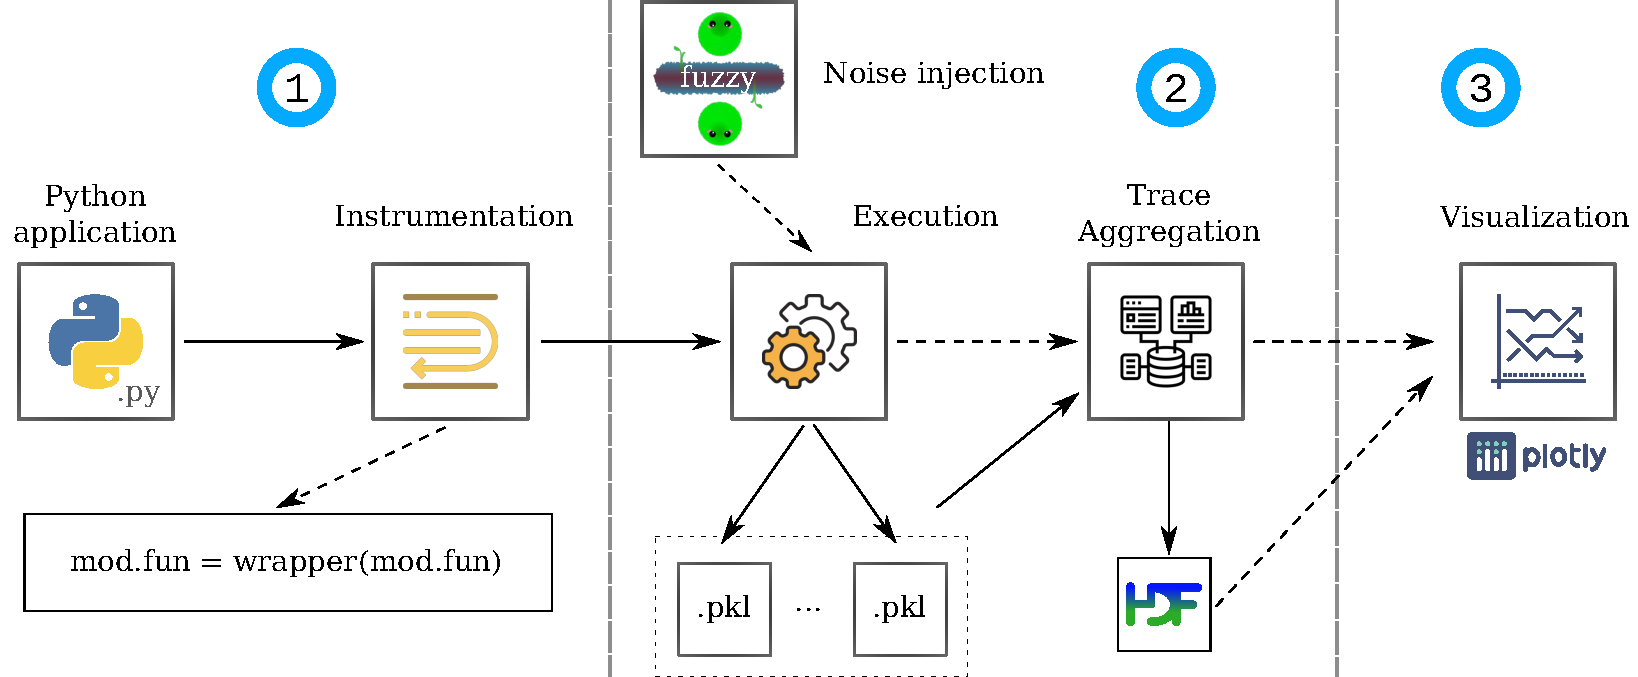
\includegraphics[width=\linewidth]{figure/workflow.pdf}
    \caption{Pytracer workflow \tristan{move the execution and noise injection to step 2}}
    \label{fig:workflow}
\end{figure}

\subsection{Python code instrumentation}

%\tristan{``Instrumentation" should appear in Figure 1}


\pytracer dynamically instruments Python modules
without requiring source code modifications in the application.
To do so, it creates a new, instrumented version of each module that preserves its original attributes so that the original application can transparently use it.
By default, \pytracer instruments all the attributes
in a given module \tristan{not only the functions?} \Yohan{No, you can have class definitions or instances that need to be wrapped}, except the special ones of the form \texttt{\_\_*\_\_}.
However, some attributes are not writable; in this case, \pytracer preservers the original attributes and warns the user. The user can also restrict the list of attributes to trace through
an inclusion/exclusion mechanism. The main advantage of this instrumentation approach is the lack of required modification in the application source code, in contrast with decorator-based approaches, which enable instrumentation in read-only environments such as Singularity containers or HPC clusters.


\subsubsection{Intercepting module import}

Python loads modules through an import mechanism triggered by the \texttt{import} keyword, using two objects: \texttt{finders} and \texttt{loaders}.
The \texttt{finder} is responsible for finding the package (or 
namespace\footnote{Python distinguishes between \texttt{regular} and \texttt{namespace} packages.
A regular package is a directory that contains a \_\_init\_\_.py file and potentially subdirectories (sub-packages) 
that contain themselves a \texttt{\_\_init\_\_.py} file and so on recursively. 
The package hierarchy follows those of the directory. 
Namespace packages introduced in Python 3.3 (\href{https://www.python.org/dev/peps/pep-0420/}{PEP 420}) do not contain an
\_\_init\_\_.py file and allow for flexible directory structures. Hence, parts of the package can be located in zip files, on the network, or in separated directories. There are no functional differences between both types of packages.}) from its fully qualified name, whether it is located on the local storage, such as standard packages installed through the pip package manager, or on a distant server.
\texttt{Finders} do not load the modules; they return a specification (\texttt{spec} object) encapsulating 
information on where to find it and how to load it.
The \texttt{loader} creates and initializes a module object, filling the import-related attributes 
such as \texttt{\_\_spec\_\_}. 
Then, the \texttt{loader} executes the module and populates its namespace. Finally, the module is bound to its import name in the \texttt{sys.modules} dictionary.


Python implements default \texttt{finder} and \texttt{loader} classes and search paths for importing a module, but it also provides a way to create custom \texttt{finder} and \texttt{loader} classes.
To register a new \texttt{finder} class, one needs to add it to the \texttt{sys.meta\_path} list.
When Python encounters an \texttt{import} statement, it first looks for a binding in the \texttt{sys.modules}
and then iterates over \texttt{sys.meta\_path}.
Python queries each \texttt{finder} class successively until it finds the module or reaches the end of the list, raising a \texttt{ModuleNotFoundError}. Then, \pytracer adds a custom \texttt{finder} class at the head of the list that intercepts
the module import and creates the module with a custom \texttt{loader} class.

\pytracer's \texttt{loader} class first loads the original module then copies it as a new instance of the \texttt{ModuleType} class. It then calls the appropriate instrumentation function for each module attribute depending on its type (function, class, or instances). Next, \pytracer replaces the original module with its instrumented counterpart in the \texttt{sys.modules} map once it has instrument all the attributes. Hence, the calling convention remains unchanged, and the application will transparently call the instrumented module. Finally, Pytracer updates all references to the original module that an object may hold. For example, functions have a \texttt{\_\_globals\_\_} attribute that contains references to internal objects that the function needs. Since those references point to non-instrumented objects, Pytracer must update them.
\tristan{is the non-instrumented version ever added to sys.modules? If so, could this lead to race conditions? If not, replace with ``adds the instrumented module to the sys.modules map"}. 
\Yohan{Yes, it replaces the original module. You can't have a race-condition since sys.modules is a dict with only one value for a given key. The trick is that the wrapped module keeps a reference to the original module, it's just that this reference is invisible for the others object since it's not in sys.modules and globals. By the way, Pytracer needs to update all possible references that original objects may hold, like functions in \_\_dict\_\_ attributes or locals references in \_\_globals\_\_ for example.}

% \pytracer intercepts the modules loaded with the \texttt{Finder} and \texttt{Loader} mechanisms \tristan{is it restrictive? Are there other mechanisms?}.
% The Finder searches the loader of a module that is being imported while the 
% Loader loads and initializes the module. \pytracer adds \tristan{overrides?} a new Finder and Loader on top of the default ones
% to intercept imports and to instrument modules selected by the user. This mechanism allows returning 
% the original module in the instrumentation code and returning the instrumented module in the targeted application
% without modifying its actual code.

\subsubsection{Instrumenting module functions}

Module functions are the most straightforward case to treat.
For each function, \pytracer's loader class creates a wrapper function, dynamically compiles it with the compile builtin function, and substitutes it for the original module function.
However, we cannot apply this technique to callable class instances, i.e., class instances that have the \texttt{\_\_call\_\_} attribute but are not of the \texttt{FunctionType} type. Indeed, applying the wrapper technique would 1) modify the type of the class instance to \texttt{FunctionType}, which could cause syntactic and semantic bugs, and 2) mask class attributes, leading to \texttt{AttributeError} exceptions.
To overcome this issue, \pytracer overrides the \texttt{\_\_call\_\_} attribute with the wrapper function when possible. When the \texttt{\_\_call\_\_} attribute is not writable,  Pytracer does not instrument the class and returns a warning. 
Listings~\ref{fig:wrapper_creation} and ~\ref{fig:generic_wrapper} show \pytracer's wrapper creation function.

\tristan{add docstrings to all Python code examples and clarify captions accordingly: you don't need to explain the meaning of each attribute in the caption if it's in the docstring. The caption can focus on the main functionality, reusing the text currently in 3.1.5.}
\Yohan{TODO}

Listing~\ref{fig:wrapper_creation} shows how functions are instrumented.
This function takes as inputs the information about the function to instrument (module name and full qualified name),
the function itself, and the actual name of the function. It then creates a wrapper around the actual wrapper
(\texttt{generic\_wrapper}) that will dump the values. Instead of passing the function, we pass the function's identifier, which is a unique 64-bits integer that references each Python object. This identifier is available
with the \texttt{id} builtin function. it allows to get rid of aliases and to avoid instrumenting functions twice. 

Listing~\ref{fig:generic_wrapper} shows what the instrumented code does. 
It first unpacks the function's information to get the function's identifier to retrieve the original function.
Then arguments are bound by creating a mapping from positional and keyword arguments to parameters, avoiding conflicts and mispositioning. It also allows getting names of arguments for the visualization.
Once bound, the \texttt{inputs} function dumps the arguments in the pickle file.
Finally, Pytracer calls the function with the correct arguments, dumps the result, and returns it.

%
% we can employ a case by case strategy depending on the class (i.e. numpy ufunc) or simply ignore
% the instrumentation and let the original one.
% \tristan{add a sentence to explain how callable instances are instrumented}




\begin{listing}
    \centering
\begin{lstlisting}[language=Python,style=customPython]
def get_wrapper_function(function_module, function_qualified_name, function, function_wrapper_name):
    function_id = id(function)
    info = (function_id, function_module, function_qualified_name)
    wrapper_code = f"""
    def {function_wrapper_name}(*args, **kwargs):
        return generic_wrapper({info},*args,**kwargs)"""
    return wrapper_code
\end{lstlisting}
    \caption{Function to create the instrumented version of a function. 
    This function returns the instrumented function as a string (\texttt{wrapper\_code}) that 
    will be turned into a Python object with the \texttt{compile} built-in function.}
    \label{fig:wrapper_creation}
\end{listing}


\begin{listing}
    \centering
\begin{lstlisting}[language=Python,style=customPython,]
def generic_wrapper(self, info, *args, **kwargs):
    fid, fmodule, fname = info
    function = original_function_cache.id_dict[fid]
    bind = Binding(function, *args, **kwargs)
    stack = self.backtrace()
    time = elements()
    self.inputs(time=time,
                module_name=fmodule,
                function_name=fname,
                function=function,
                args=bind.arguments,
                backtrace=stack)
    outputs = function(*bind.args, **bind.kwargs)
    self.outputs(time=time,
                 module_name=fmodule,
                 function_name=fname,
                 function=function,
                 args=outputs,
                 backtrace=stack)
    return outputs
\end{lstlisting}
    \caption{\pytracer's wrapper function. 
    The \texttt{original\_function\_cache} maintains a mapping between the original function and its identifier (available through 
    \texttt{id} built-in function). Once the original function retrieved, the arguments are saved to the traces (through function 
    \texttt{self.inputs}). The actual function is called and the result is saved (function \texttt{self.outputs}) then returned.
    }
    \label{fig:generic_wrapper}
\end{listing}


\subsubsection{Instrumenting classes}

\pytracer instruments classes by wrapping their callable attributes as described previously. 
This instrumentation preserves class types, avoiding type mismatches in the instrumented application.
However, some classes, in particular base types, contain read-only attributes that cannot be instrumented. 
By default, \pytracer returns a warning when it encounters such classes, 
but it treats NumPy's universal functions (\texttt{ufuncs}) specifically since they are ubiquitous in scientific computing. 
NumPy's \texttt{ufuncs} are vectorized element-wise operators that apply to multidimensional arrays. 
In particular, all the element-wise elementary mathematical functions are \texttt{ufuncs}.  
To increase performance, \texttt{ufuncs} are implemented in C, which prevents their instrumentation using the technique described previously. 
Instead, \pytracer uses NumPy's \texttt{frompyfunc} helper function to create an instrumented \texttt{ufunc} that wraps the original one.
This approach works in many cases but it requires the instrumented function to return objects of type \texttt{PyObject}, 
which may create errors (Listing~\ref{fig:numpy_array_index_issue}). 
As a last resort, the user may disable \texttt{ufunc} tracing in Pytracer.


\subsubsection{Instrumenting iterators}
In functional programming, iterators traverse containers lazily, meaning that the next element in the sequence is only computed when the application uses it. This technique allows for the manipulation of virtually infinite sequences within finite memory. However, it implies no complete mapping of the container returned by an iterator in memory since the application computes each element on the fly. Therefore, iterators are not serializable, and \pytracer cannot save them to output traces. 
A workaround would be to convert iterators into explicit containers and then return a new iterator on the explicit container. However, this would increase the memory footprint, possibly significantly, and \pytracer, therefore, does not instrument iterators.

\begin{listing}
\begin{minipage}[t]{0.4\linewidth}
    \begin{lstlisting}[language=Python,style=customPython]
>>> import numpy as np
>>> x = np.array(range(10))
>>> index = np.array([1,-1],dtype=int)
>>> x[index]
>>> array([1, 9])
    \end{lstlisting}
\end{minipage}
\begin{minipage}[t]{0.4\linewidth}
    \begin{lstlisting}[language=Python,style=customPython]
>>> import numpy as np
>>> x = np.array(range(10))
>>> index = np.array([1,-1], dtype=object)
>>> x[index]
Traceback (most recent call last):
  File "<stdin>", line 1, in <module>
IndexError: arrays used as indices must be of integer (or boolean) type
    \end{lstlisting}
\end{minipage}
\caption{Illustration of the issue of using \texttt{frompyfunc} function to convert function to \texttt{ufunc}. Left: original code. Right: instrumented code. 
\tristan{This needs more explanation: where is the ufunc, what is the type returned by the original ufunc, and why does it crash in the instrumented version.} \Yohan{TODO}}
    \label{fig:numpy_array_index_issue}
\end{listing}

\subsection{Detecting numerical instabilities}

\pytracer detects numerical instabilities by computing summary statistics across multiple application executions perturbed with numerical noise. While \pytracer's instrumentation, trace aggregation, and visualization work with various types of numerical noise, we experimented primarily with Monte-Carlo Arithmetic (MCA) as it is the most accurate model for floating-point errors.

\subsubsection{Noise injection}
\label{sec:fuzzy}


We enable MCA in Python programs via Verificarlo~\cite{verificarlo}, a clang-based compiler~\cite{lattner2008llvm} that replaces floating-point operations by a generic call to a configurable floating-point model. Several floating-point models, also called backends, are available~\cite{chatelain2019automatic,chatelain2019outils}.
We leverage the fuzzy~\cite{kiar2020comparing} environment, a collection of software tools recompiled with Verificarlo. In particular, fuzzy provides MCA-instrumented versions of the Python interpreter and BLAS, LAPACK, NumPy, SciPy, and scikit-learn, which allows for MCA injection perturbations to a wide range of existing scientific Python programs. Fuzzy is available in Verificarlo's GitHub organization at \href{https://github.com/verificarlo/fuzzy}{\url{github.com/verificarlo/fuzzy}} and provides Docker images for each MCA-enabled tool.

% As the time of writing this article, fuzzy provides 5 levels of instrumentation (each level N including the lower levels):
% \begin{enumerate}
%     \item BLAS + LAPACK
%     \item Python interpreter
%     \item Numpy
%     \item SciPy
%     \item Scikit-learn
% \end{enumerate}

\subsubsection{Trace format}

\pytracer stores the traces in the pickle format, a compressed binary Python format to serialize Python objects.
The main advantages of the pickle format compared to other serialization approaches such as marshal or JSON are its ability to serialize most Python objects and its native compression.  In addition, pickle writes Python objects sequentially according to their serialization order, which preserves the temporal ordering required by subsequent trace analyses.

Traces record numerical values at the granularity of a function. When the application invokes a function, \pytracer saves a call input object containing contextual information (function's name, module's function, stacktrace) and the values of the function arguments. When the function returns, \pytracer saves a similar call output object containing the returned value. 


\subsubsection{Trace aggregation}

Once traces are available, \pytracer sequentially parses them and computes the mean, standard deviation, and the number of significant digits (using Equation~\ref{eq:sig-digits}) of all saved values. Pytracer saves these summary statistics in an HDF5 file, a hierarchical format that facilitates browsing during the visualization. This operation critically relies on the ordering of call input and output objects in the traces. Furthermore, it assumes that the application is deterministic, and in particular, assumes it is single-threaded and that the control flow does not depend on a random state. Techniques to overcome this limitation are discussed in the discussion section.

\begin{figure}
    \centering
    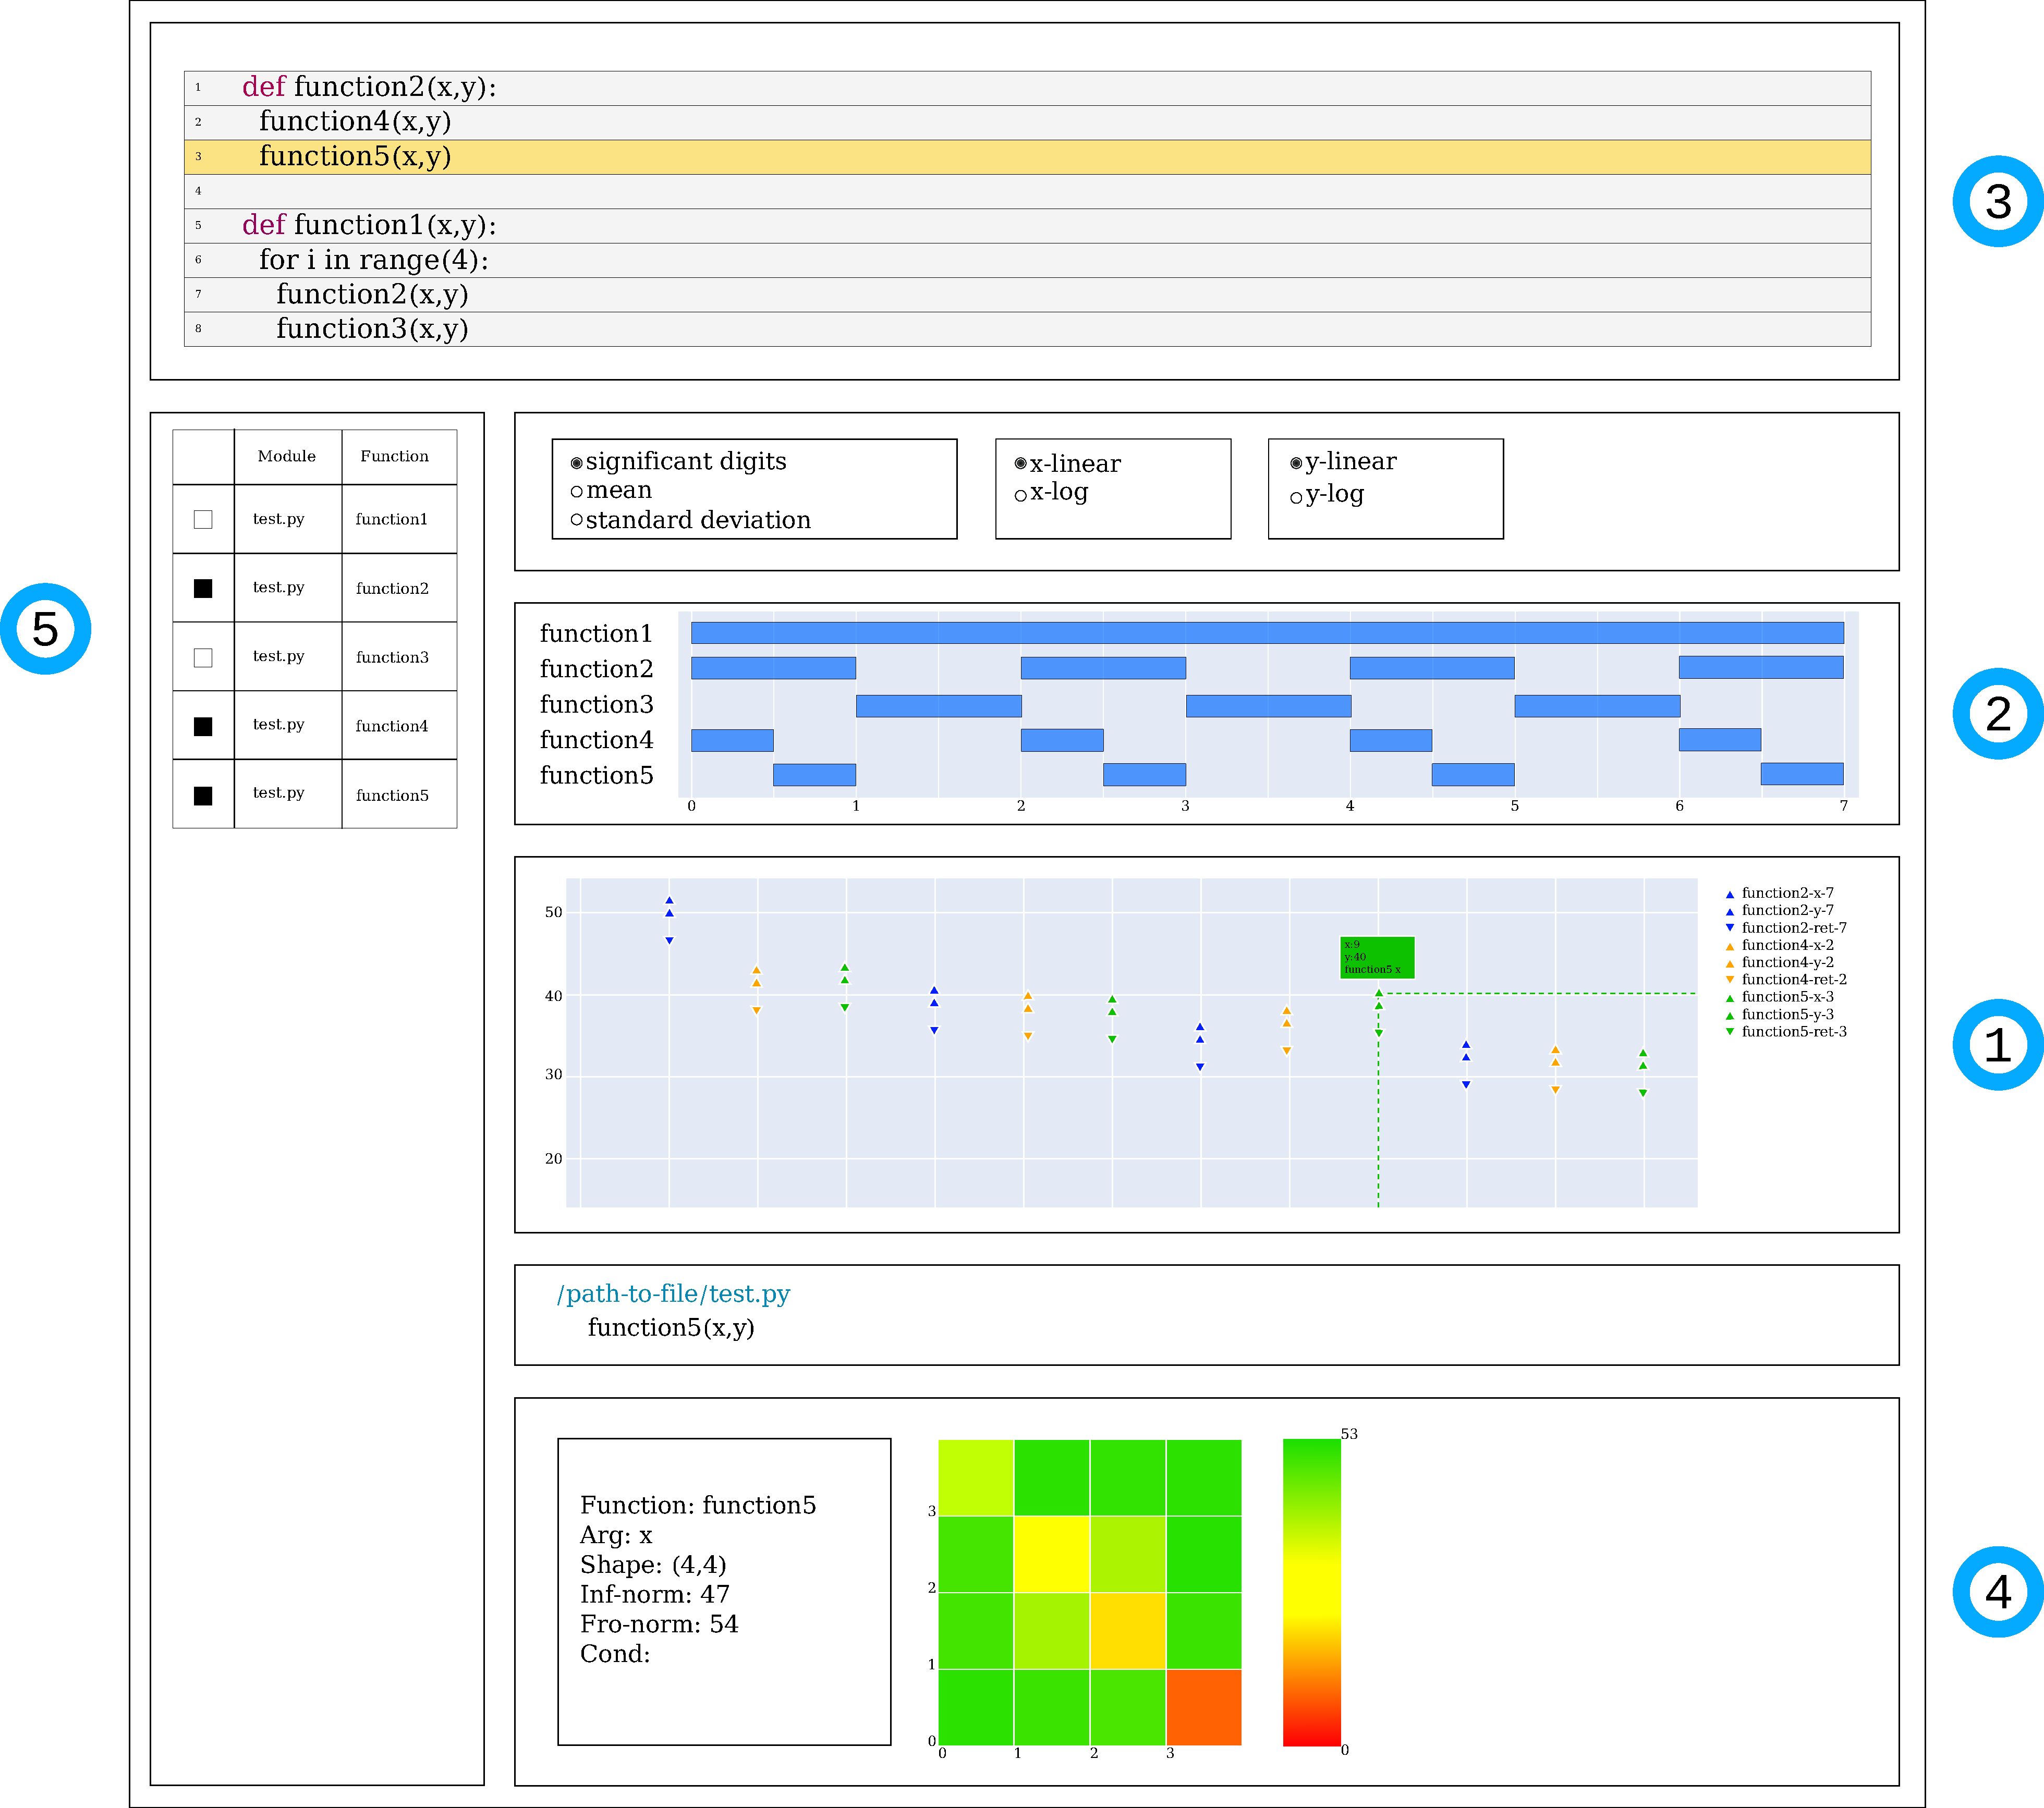
\includegraphics[width=\textwidth]{figure/pytracer_layout.pdf}
    \caption{Pytracer visualization layout.}
    \label{fig:visu-layout}
\end{figure}


To aggregate traces, \pytracer successively unpickles call objects in each trace, checks
that the call objects refer to the same function and stacktrace, and terminates the parsing otherwise.
For each matching call object, \pytracer stores function arguments or returned values in a NumPy array to compute statistics. 
For compound objects such as tuples, dictionaries, or objects, it recursively parses the fields until finding
numeric types or NumPy arrays of numeric types.

\subsection{Interactive visualization}
The third main component of \pytracer is its interactive trace visualizer built with Plotly Dash~\cite{plotly}, a Python framework for web visualization.
Plotly Dash abstracts the low-level details of web applications in a highly customizable development interface allowing to offload heavy computations to a server. 
Figure~\ref{fig:visu-layout} presents the general layout of the \pytracer visualizer, divided into five sub-components:
\begin{enumerate}
 \item Timeline view: This view displays the values of each input and output for a given function at a given invocation. By default, \pytracer shows the number of significant digits computed across the traces, but the user can switch to the mean or the standard deviation. The visualizer uses an upper triangle for inputs and a down triangle to differentiate inputs from outputs. \pytracer internally represents all values as NumPy arrays.    In the case of non-scalar values or types that cannot be trivially cast into NumPy arrays, \pytracer splits the value into several variables. Hence, \pytracer will transform a class containing $n$ floating-point parameters into $n$ variables. Each variable is prefixed with the original value and postfixed with the name of the parameter. 
    Finally, for non-scalar values (vectors or matrices), \pytracer shows the average elements for non-scalar values (like vectors or matrices). non-scalar values can be inspected with the Zoom view (see below).
 \item Gantt chart view: This view displays the call graph as a Gantt chart representing the instrumented functions. Each function call is represented with a bar starting and ending at the function call and return.
    The caller/callee relation is then determined by looking at the time overlaps.
    For example, in the figure, \texttt{function1} calls \texttt{function2} that itself calls \texttt{function4} and \texttt{function5}. 
    This view provides insights on the calling context for each function since different parents functions can call the same function, which may influence numerical stability. 
 \item  Source code view: This view displays the source code file of the variable hovered in the timeline view. 
 \item Zoom view: This view allows closely examine non-scalar values, which is helpful to see local differences that might be masked by the averaging done in the timeline view. For example, a matrix can have instabilities around its diagonal but not in other regions.
    The visualizer also provides metrics about the value, such as the array shape, infinite norm, or condition number.
\item  Functions list view: This view allows the user to select the functions to plot in the timeline view.
\end{enumerate}

\section{Numerical evaluations}

We evaluated \pytracer on widely-used Python libraries, namely SciPy, scikit-learn, and PyAFQ, demonstrating its scalability and usability for real-world Python programs. 
SciPy is a Python-based ecosystem of open-source software for mathematics, science, and engineering, including NumPy.
Scikit-learn is an open-source Python library for machine learning built upon SciPy.
PyAFQ is a software package focused on automated delineation of the major fiber tracts in individual human brains, and quantification of the tissue properties within the tracts.
For SciPy and scikit-learn, we traced each application five times, having activated MCA in the Python interpreter, BLAS, LAPACK, NumPy, SciPy, and scikit-learn. We repeated the experiment with two MCA modes, Random Rounding (RR) and Full MCA, and having enabled or disabled the instrumentation of NumPy's universal functions (\texttt{ufuncs}), resulting in 4 experiments for each application. We used the default virtual precision in Verificarlo, namely 24 bits for single-precision floating-point values and 53 bits for double-precision values, which simulates machine error. For each library, we executed the software tests provided in the GitHub repositories.

\subsection{Results overview}

Tables~\ref{tab:pytracer_scipy_results_summary} and~\ref{tab:pytracer_sklearn_results_summary} summarize 
the outcome of \pytracer experiments on SciPy and scikit-learn.
Each table reports on the tracing and trace aggregation steps with three possible outcomes: green for success, red for numerical error in the application, and orange for errors in the fuzzy noise injection or due to the instrumentation of NumPy \texttt{ufuncs}. Overall, the tracing and parsing of SciPy and scikit-learn tests in Random Rounding mode and without \texttt{ufunc} instrumentation was entirely successful (tracing and parsing steps) for 31/40 tests. The remaining tests failed due to numerical errors in the libraries, which we discuss hereafter. The instrumentation with Full MCA is more invasive and reduced the number of successful executions without \texttt{ufunc} instrumentation to 11/40.  The instrumentation of \texttt{ufuncs} also reduced the success rate substantially, to 17/40 in Random Rounding mode and to 8/40 in Full MCA. 

\begin{table}[]
    \centering
    \begin{tabular}{|ll|c|c|c|c||c|c|c|c|}
    \hline
    \multicolumn{2}{|c}{ \multirow{3}{*}{Application} } & \multicolumn{4}{|c||}{Random Rounding (RR)} & \multicolumn{4}{c|}{Full MCA} \\\cline{3-10}
         &   & \multicolumn{2}{c|}{\texttt{ufunc}} & \multicolumn{2}{c||}{no \texttt{ufunc}} & \multicolumn{2}{c|}{\texttt{ufunc}} & \multicolumn{2}{c|}{no \texttt{ufunc}} \\\cline{3-10}
    & & trace & parse &  trace & parse & trace & parse & trace & parse \\
    \hline
    %        &               RR                 &                 MCA               \\
    %        &  numpy         &   no numpy      &      numpy      &     no numpy    \\
    %        & run   & parse  &  run   &  parse &  run   & parse  & run    & parse  \\
    
    \multicolumn{1}{|c|}{ \multirow{3}{2em}{ \rotatebox{90}{FFT} } }
    & discrete\_cosine\_transform & \valid & \valid & \valid & \valid & \valid & \valid & \warn & \cross \\ 
    \multicolumn{1}{|c|}{} & fft\_1D & \warn & \valid & \valid & \valid & \warn & \cross & \warn & \cross \\
    \multicolumn{1}{|c|}{} & fft\_2D & \valid & \valid & \valid & \valid & \valid & \valid & \valid & \valid \\
    \hline 
    \multicolumn{1}{|c|}{  \multirow{5}{2em}{ \rotatebox{90}{Interpolation} } }
    & interpolation\_1D & \valid & \valid & \valid & \valid & \valid & \cross & \warn & \cross  \\
    \multicolumn{1}{|c|}{} & multivariate\_data & \valid & \valid & \valid & \valid & \valid & \cross & \warn & \cross \\
     \multicolumn{1}{|c|}{} & bspline & \valid & \valid & \valid & \valid & \valid & \valid & \valid & \valid \\
     \multicolumn{1}{|c|}{} & spline\_1D & \warn & \valid & \valid & \cross & \warn & \cross & \warn & \cross \\
     \multicolumn{1}{|c|}{} & spline\_2D & \warn & \valid & \valid & \valid & \warn & \cross & \warn & \cross \\
    \hline
     \multicolumn{1}{|c|}{ \multirow{12}{2em}{ \rotatebox{90}{Optimization} } }
    & broyden\_fletcher\_goldfarb\_shanno & \valid & \valid & \valid & \valid & \valid & \valid & \valid & \valid \\
     \multicolumn{1}{|c|}{} & global\_optimization & \warn & \valid & \warn & \valid & \warn & \cross & \cross & \cross \\
    \multicolumn{1}{|c|}{}  & slsqp & \warn & \valid & \valid & \valid & \warn & \cross & \valid & \cross \\
     \multicolumn{1}{|c|}{} & least\_square\_minimization & \warn & \valid & \valid & \valid & \warn & \cross & \valid & \valid \\
     \multicolumn{1}{|c|}{} & nelder\_mead\_simplex & \valid & \valid & \valid & \valid & \valid & \valid & \valid & \valid \\
     \multicolumn{1}{|c|}{} & newton\_conjugate\_gradient & \valid & \cross & \valid & \cross & \valid & \cross & \valid & \cross \\
     \multicolumn{1}{|c|}{} & root\_finding\_large\_preconditionned & \valid & \cross & \valid & \cross & \warn & \cross & \valid & \cross \\
    \multicolumn{1}{|c|}{}  & root\_finding\_large & \warn & \valid & \valid & \cross & \valid & \cross & \valid & \cross \\
     \multicolumn{1}{|c|}{} & root\_findings & \warn & \valid & \valid & \valid & \warn & \valid & \warn & \cross \\
    \multicolumn{1}{|c|}{}  & trust\_region\_exact & \valid & \valid & \valid & \valid & \valid & \valid & \valid & \valid \\
     \multicolumn{1}{|c|}{} & trust\_region\_truncated\_generalized\_lanczos & \valid & \valid & \valid & \valid & \valid & \valid & \valid & \valid \\
    \multicolumn{1}{|c|}{}  & trust\_region\_newton\_conjugate\_gradient & \valid & \valid & \valid & \valid & \valid & \valid & \valid & \valid \\
    \hline
    \end{tabular}
    \caption{\pytracer execution summary on SciPy tests.\\RR: Random Rounding. \texttt{ufunc}: instrumentation of NumPy \texttt{ufuncs}. trace: outcome of \pytracer tracing, parse: outcome of \pytracer trace parsing and aggregation.  \valid: successful run, \warn: error in fuzzy noise injection or due to the instrumentation of NumPy \texttt{ufuncs}, \cross: numerical error.}
    \label{tab:pytracer_scipy_results_summary}
\end{table}

\begin{table}[]
    \centering
    \begin{tabular}{|c|c|c|c|c||c|c|c|c|}
    \hline
    \multirow{3}{5em}{Application} & \multicolumn{4}{|c||}{Random Rounding (RR)} & \multicolumn{4}{|c|}{Full MCA} \\\cline{2-9}
                & \multicolumn{2}{|c|}{\texttt{ufunc}} &  \multicolumn{2}{|c||}{no \texttt{ufunc}} & \multicolumn{2}{|c|}{\texttt{ufunc}} & \multicolumn{2}{|c|}{no \texttt{ufunc}} \\\cline{2-9}
                & trace & parse &  trace & parse & trace & parse & trace & parse \\
    \hline
    %        &               RR                 &                 MCA               \\
    %        &  numpy         &   no numpy      &      numpy      &     no numpy    \\
    %        & run   & parse  &  run   &  parse &  run   & parse  & run    & parse  \\
    Adaboost & \warn & \valid & \valid & \valid & \warn & \cross & \cross & \cross \\
    Bayesian Ridge Regression & \warn & \valid & \valid & \valid & \cross & \cross & \cross & \cross \\
    Online classifier comparison & \valid & \valid & \valid & \valid & \cross & \cross & \cross & \cross  \\
    Cluster Iris & \valid & \valid & \valid & \valid & \valid & \cross & \valid & \cross \\
    Covariance estimation & \valid & \cross & \valid & \cross & \cross & \cross & \valid & \cross \\
    Decision Tree Regression & \valid & \valid & \valid & \valid & \valid & \cross & \valid & \cross \\
    Digits Classification & \warn & \valid & \valid & \valid & \warn & \cross & \cross & \cross \\
    Face Recognition & \cross & \valid & \cross & \valid & \cross & \cross & \cross & \cross \\
    L1 Penalty & \warn & \valid & \valid & \valid & \warn & \cross & \valid & \valid \\
    Lasso and elastic net & \warn & \valid & \valid & \valid & \warn & \cross & \valid & \cross \\
    Separating hyperplan & \valid & \valid & \valid & \valid & \valid & \cross & \valid & \cross \\
    MNIST classification & \warn & \valid & \valid & \valid & \valid & \cross & \valid & \valid \\
    Multitask Lasso & \warn & \valid & \valid & \valid & \warn & \cross & \valid & \valid \\
    Orthogonal matching & \warn & \valid & \valid & \valid & \cross & \valid & \cross & \valid \\
    PCA decomposition & \warn & \valid & \valid & \valid & \warn & \cross & \valid & \cross \\
    Robust Linear Regression & \valid & \valid & \valid & \valid & \warn & \cross & \valid & \cross \\
    Segmentation toy & \warn & \valid & \valid & \cross & \warn & \cross & \cross & \cross \\
    SVM & \valid & \valid & \valid & \valid & \valid & \cross & \valid & \cross \\
    Tomography & \warn & \valid & \valid & \cross & \warn & \cross & \cross & \cross \\
    Weighted samples & \valid & \valid & \valid & \valid & \valid & \cross & \valid & \cross \\
    \hline
    \end{tabular}
    \caption{\pytracer execution summary on Scikit-learn tests. \\RR: Random Rounding. \texttt{ufunc}: instrumentation of NumPy \texttt{ufuncs}. trace: outcome of \pytracer tracing, parse: outcome of \pytracer trace parsing and aggregation.  \valid: successful run, \warn: error in fuzzy noise injection or due to the instrumentation of NumPy \texttt{ufuncs}, \cross: numerical error.}
    \label{tab:pytracer_sklearn_results_summary}
\end{table}



\subsubsection{Effect of MCA modes}
\label{sec:impact_mca_modes}
Random Rounding perturbs only the result of a floating-point operation, while Full MCA mode perturbs both the inputs and the operation's result. 
Therefore, full MCA mode may trigger catastrophic cancellations while Random Rounding only introduces round-off errors which generally have a lesser impact.
Moreover, Random Rounding preserves exact operations, i.e., operations where the result can be exactly represented on the virtual precision, while Full MCA does not.

\pytracer can only aggregate traces obtained from the same control flow path. In particular, program branches triggered by an unstable floating-point comparison lead to different control flows and result in parsing errors. 
For example, comparing a residual error to a strict threshold in an iterative scheme or comparing the distance between two points generally results in unstable branches. 
With Full MCA, even exact values such as integers represented with floating-point values are perturbed, leading to many execution failures. For instance,  the \texttt{fft1} test from SciPy raised an \texttt{ValueError: operands could not be broadcast together with shapes (601,) (600,)} error due to an array shape mismatch. A closer inspection showed that one of the arrays involved in the error is created with the NumPy function \texttt{linspace} that itself calls function \texttt{arange} (Listing~\ref{fig:pyarray_range_code}). As can be seen in lines  3174-3178, the array size is stored in a floating-point value which will therefore be perturbed in Full MCA mode, as shown in Table~\ref{tab:mca_result_linspace}, resulting in array sizes that fluctuate
between N and N+1. 
It is worth noting that 78\% of execution issues encountered in Full MCA mode without \texttt{ufunc} instrumentation
are due to this type of ``typing" errors. While they do not lead to any numerical issue, such typing errors should still be fixed to preserve code quality. We provide solutions to help MCA better work with those cases in the discussion section.

\tristan{Check this last sentence, we need to provide some sort of recommendations}. \tristan{how about opening a PR in numpy to fix this error?}
\Yohan{For this case, they use the math.ceil to correctly round the number, I think the fix is more on the MCA side to
correctly handle exact number than on the NumPy side.}


% \begin{figure}
%     \begin{lstlisting}[language=Python,style=customPython,numbers=left, firstnumber=11]
% # Number of sample points
% N = 600
% # sample spacing
% T = 1.0 / 800.0
% x = np.linspace(0.0, N*T, N, endpoint=False)
% y = np.sin(50.0 * 2.0*np.pi*x) + 0.5*np.sin(80.0 * 2.0*np.pi*x)
% yf = fft(y)
% w = blackman(N)
% ywf = fft(y*w)
%     \end{lstlisting}
%     \label{fig:fft1_code}
% \caption{Code snippet from \texttt{fft\_1D} illustrating issue arising when using Full MCA mode.
% Line 19 raises \texttt{ValueError: operands could not be broadcast together with shapes (601,) (600,)} since
% arrays \texttt{y} and \texttt{w} do not have the same shape. This is due to random errors introduces by 
% Full MCA mode in the \texttt{linspace} function.
% }
% \end{figure}

% \begin{figure}
%     \begin{lstlisting}[language=Python,style=customPython,numbers=left, firstnumber=1, mathescape=true]
% def linspace(start, stop, num=50, endpoint=True, retstep=False, dtype=None,
%              axis=0):
%     num = operator.index(num) // 3 $\lstsetnumber{\ldots}$
%     ...$\lstresetnumber\setcounter{lstnumber}{5}$
%     div = (num - 1) if endpoint else num // 6  $\lstsetnumber{\ldots}$
%     ...$\lstresetnumber\setcounter{lstnumber}{13}$
%     delta = stop - start // 14
%     y = _nx.arange(0, num, dtype=dt).reshape((-1,) + (1,) * ndim(delta)) // 15
%     \end{lstlisting}
%     \label{fig:linspace_code}
% \caption{Code snippet from \texttt{linspace} function from numpy package. 
%     It uses the \textit{arange} function implemented as a Cython function (fig.~\ref{fig:pyarray_range_code}) to create the array. 
% }
% \end{figure}
    

\begin{listing}
    \begin{lstlisting}[language=C,style=customC,numbers=left, firstnumber=3163, mathescape=true]
/*NUMPY_API
  Arange,
*/
NPY_NO_EXPORT PyObject *
PyArray_Arange(double start, double stop, double step /* default 1 */, int type_num) 
{
    npy_intp length; 
    PyArrayObject *range; $\lstsetnumber{\ldots}$
    ...$\lstresetnumber\setcounter{lstnumber}{3173}$
    double delta, tmp_len; $\lstsetnumber{\ldots}$
    ...$\lstresetnumber\setcounter{lstnumber}{3176}$
    delta = stop - start; 
    tmp_len = delta/step; $\lstsetnumber{\ldots}$
    ...$\lstresetnumber\setcounter{lstnumber}{3189}$
        length = _arange_safe_ceil_to_intp(tmp_len); $\lstsetnumber{\ldots}$
    ...$\lstresetnumber\setcounter{lstnumber}{3201}$
    range = (PyArrayObject *)PyArray_New(&PyArray_Type, 1, &length, type_num, $\lstsetnumber{}$
                        NULL, NULL, 0, 0, NULL);
    \end{lstlisting}
\caption{Source code of the \texttt{PyArray\_Range} Cython function called by NumPy function \texttt{linspace} to create an array of equally spaced elements. The temporary array size assigned in line 3178 is stored as a floating-point value and is therefore perturbed in Full MCA mode, leading to differences amplified by the use of ceil rounding at line 3190 and resulting in different array sizes across MCA-perturbed executions. See also Table~\ref{tab:mca_result_linspace}.}
    \label{fig:pyarray_range_code}

\end{listing}

    
\begin{table}[]
    \centering
    \footnotesize
    \begin{tabularx}{{\textwidth}}{cccc>{\centering\arraybackslash}X>{\centering\arraybackslash}X>{\centering\arraybackslash}X}
                \thickhline
    \textbf{Mode}  & \textbf{start} & \textbf{stop} & \textbf{step} & \textbf{delta} & \textbf{tmp\_len} & \textbf{ceil(tmp\_len)}  \\
    \hline
    Exact & 0 & 600  & 1 & 600                             & 600                            & 600             \\
    RR    & 0 & 600  & 1 & 600 $\pm$ 0.0                   & 600 $\pm$ 0.0                  & 600 $\pm$ 0.0   \\
    MCA    & 0 & 600  & 1 & 599.9999999999999 $\pm$ 8e-14  & 600.0 $\pm$ 8e-14 &  600.01 $\pm$ 0.0995\\
            \thickhline

    \end{tabularx}
    \caption{Results obtained through lines 3177-3190 in Listing~\ref{fig:pyarray_range_code}. Contrary to RR mode, Full MCA mode does not preserve exact operations which leads to an array length oscillating between 600 and 601.}
    \label{tab:mca_result_linspace}
\end{table}

\subsubsection{Overall numerical quality}



\subsection{SciPy}
\label{sec:scipy_tests}

We tested Pytracer on SciPy~\cite{virtanen2020scipy} examples provided in the tutorial website section.
SciPy is organized in several libraries targeting specific computing domains.
We focused on the following packages:
\begin{itemize}
    \item \texttt{fftpack}: Fast Fourier Transform routines.
    \item \texttt{interpolate}: Interpolation and smoothing splines.
    \item \texttt{optimize}: Optimization and root-finding routines.
\end{itemize}



\subsection{Scikit learn}
\label{sec:sklearn_tests}

We tested Pytracer on Scikit-learn~\cite{pedregosa2011scikit}, a "Python module integrating a wide range of state-of-the-art machine learning algorithms for medium-scale supervised and unsupervised problems".
Scikit-learn offers a well supplied and documented list of examples that facilitates its using with Pytracer.
Among the several available examples, we choose the following representative set:
\href{https://scikit-learn.org/stable/auto_examples/ensemble/plot_adaboost_regression.html#sphx-glr-auto-examples-ensemble-plot-adaboost-regression-py}{Decision Tree Regression with AdaBoost},
\href{https://scikit-learn.org/stable/auto_examples/linear_model/plot_bayesian_ridge.html#sphx-glr-auto-examples-linear-model-plot-bayesian-ridge-py}{Bayesian Ridge Regression}, 
\href{https://scikit-learn.org/stable/auto_examples/linear_model/plot_sgd_comparison.html#sphx-glr-auto-examples-linear-model-plot-sgd-comparison-py}{Comparing various online solvers}, 
\href{https://scikit-learn.org/stable/auto_examples/linear_model/plot_sgd_comparison.html#sphx-glr-auto-examples-linear-model-plot-sgd-comparison-py}{K-means Clustering},
\href{https://scikit-learn.org/stable/auto_examples/linear_model/plot_sgd_comparison.html#sphx-glr-auto-examples-linear-model-plot-sgd-comparison-py}{Recognizing hand-written digits},
\href{https://scikit-learn.org/stable/auto_examples/decomposition/plot_faces_decomposition.html#sphx-glr-auto-examples-decomposition-plot-faces-decomposition-py}{Faces dataset decompositions},
\href{https://scikit-learn.org/stable/auto_examples/linear_model/plot_logistic_l1_l2_sparsity.html#sphx-glr-auto-examples-linear-model-plot-logistic-l1-l2-sparsity-py}{L1 Penalty and Sparsity in Logistic Regression},
\href{https://scikit-learn.org/stable/auto_examples/linear_model/plot_lasso_and_elasticnet.html#sphx-glr-auto-examples-linear-model-plot-lasso-and-elasticnet-py}{Lasso and Elastic Net for Sparse Signals},
\href{https://scikit-learn.org/stable/auto_examples/linear_model/plot_sgd_separating_hyperplane.html#sphx-glr-auto-examples-linear-model-plot-sgd-separating-hyperplane-py}{SGD: Maximum margin separating hyperplane},
\href{https://scikit-learn.org/stable/auto_examples/linear_model/plot_sparse_logistic_regression_mnist.html#sphx-glr-auto-examples-linear-model-plot-sparse-logistic-regression-mnist-py}{MNIST classification using multinomial logistic + L1},
\href{https://scikit-learn.org/stable/auto_examples/linear_model/plot_sgd_iris.html#sphx-glr-auto-examples-linear-model-plot-sgd-iris-py}{Plot multi-class SGD on the iris dataset},
\href{https://scikit-learn.org/stable/auto_examples/linear_model/plot_multi_task_lasso_support.html#sphx-glr-auto-examples-linear-model-plot-multi-task-lasso-support-py}{Joint feature selection with multi-task Lasso},
\href{https://scikit-learn.org/stable/auto_examples/linear_model/plot_omp.html#sphx-glr-auto-examples-linear-model-plot-omp-py}{Orthogonal Matching Pursuit},
\href{https://scikit-learn.org/stable/auto_examples/decomposition/plot_pca_iris.html#sphx-glr-auto-examples-decomposition-plot-pca-iris-py}{PCA example with Iris Data-set},
\href{https://scikit-learn.org/stable/auto_examples/linear_model/plot_poisson_regression_non_normal_loss.html#sphx-glr-auto-examples-linear-model-plot-poisson-regression-non-normal-loss-py}{Poisson regression and non-normal loss},
\href{https://scikit-learn.org/stable/auto_examples/cluster/plot_segmentation_toy.html#sphx-glr-auto-examples-cluster-plot-segmentation-toy-py}{Spectral clustering for image segmentation},
\href{https://scikit-learn.org/stable/auto_examples/svm/plot_separating_hyperplane_unbalanced.html#sphx-glr-auto-examples-svm-plot-separating-hyperplane-unbalanced-py}{SVM: Separating hyperplane for unbalanced classes},
\href{https://scikit-learn.org/stable/auto_examples/applications/plot_tomography_l1_reconstruction.html#sphx-glr-auto-examples-applications-plot-tomography-l1-reconstruction-py}{Compressive sensing: tomography reconstruction with L1 prior (Lasso)},
\href{https://scikit-learn.org/stable/auto_examples/linear_model/plot_tweedie_regression_insurance_claims.html#sphx-glr-auto-examples-linear-model-plot-tweedie-regression-insurance-claims-py}{Tweedie regression on insurance claims},
\href{https://scikit-learn.org/stable/auto_examples/linear_model/plot_sgd_weighted_samples.html#sphx-glr-auto-examples-linear-model-plot-sgd-weighted-samples-py}{SGD: Weighted samples}.

We used the fuzzy environment with numpy, scipy and scitkit-learn instrumented. 
We tested two perturbations modes: Random Rounding (RR) and Full MCA (MCA).




Table~\ref{tab:pytracer_sklearn_results_summary} summaries sklearn experiments with Pytracer.


% \subsubsection{Decision Tree Regression with AdaBoost}

% A decision tree is boosted using the AdaBoost.R2~\cite{drucker1997improving} 
% algorithm on a 1D sinusoidal dataset with a small amount of Gaussian noise. 
% 299 boosts (300 decision trees) is compared with a single decision tree regressor. 
% As the number of boosts is increased the regressor can fit more detail. 
% The execution with Pytracer reveals a numerical stability.

% \begin{figure}
%     \centering
%     \caption{Caption}
%     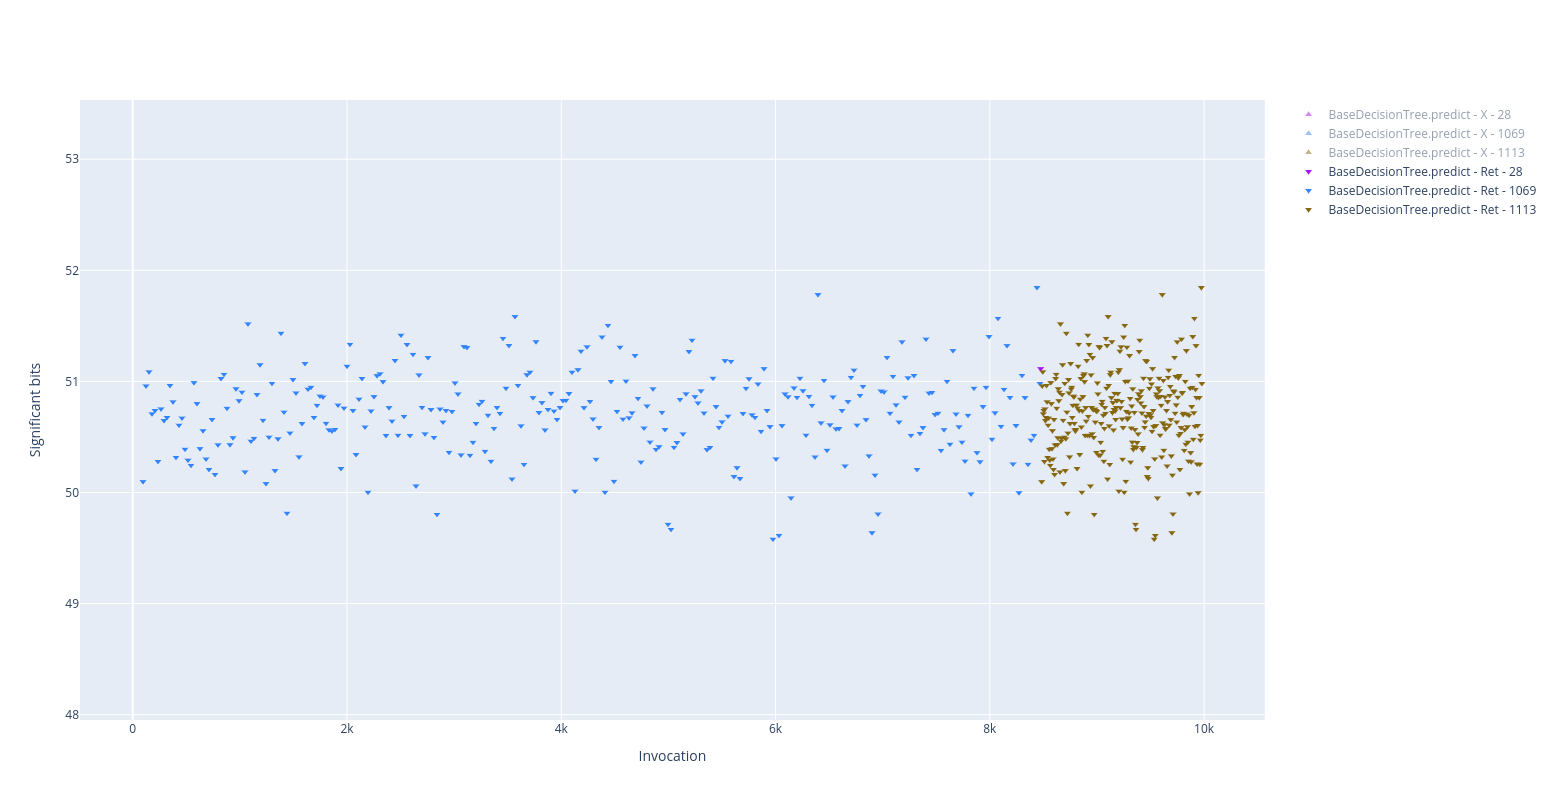
\includegraphics[width=\linewidth]{figure/adaboost/predict_adaboost_s.png}
%     \caption{Number of significant digits of predicted values array.}
%     \label{fig:adaboost_predict_s}
% \end{figure}

% \begin{figure}
%     \centering
%     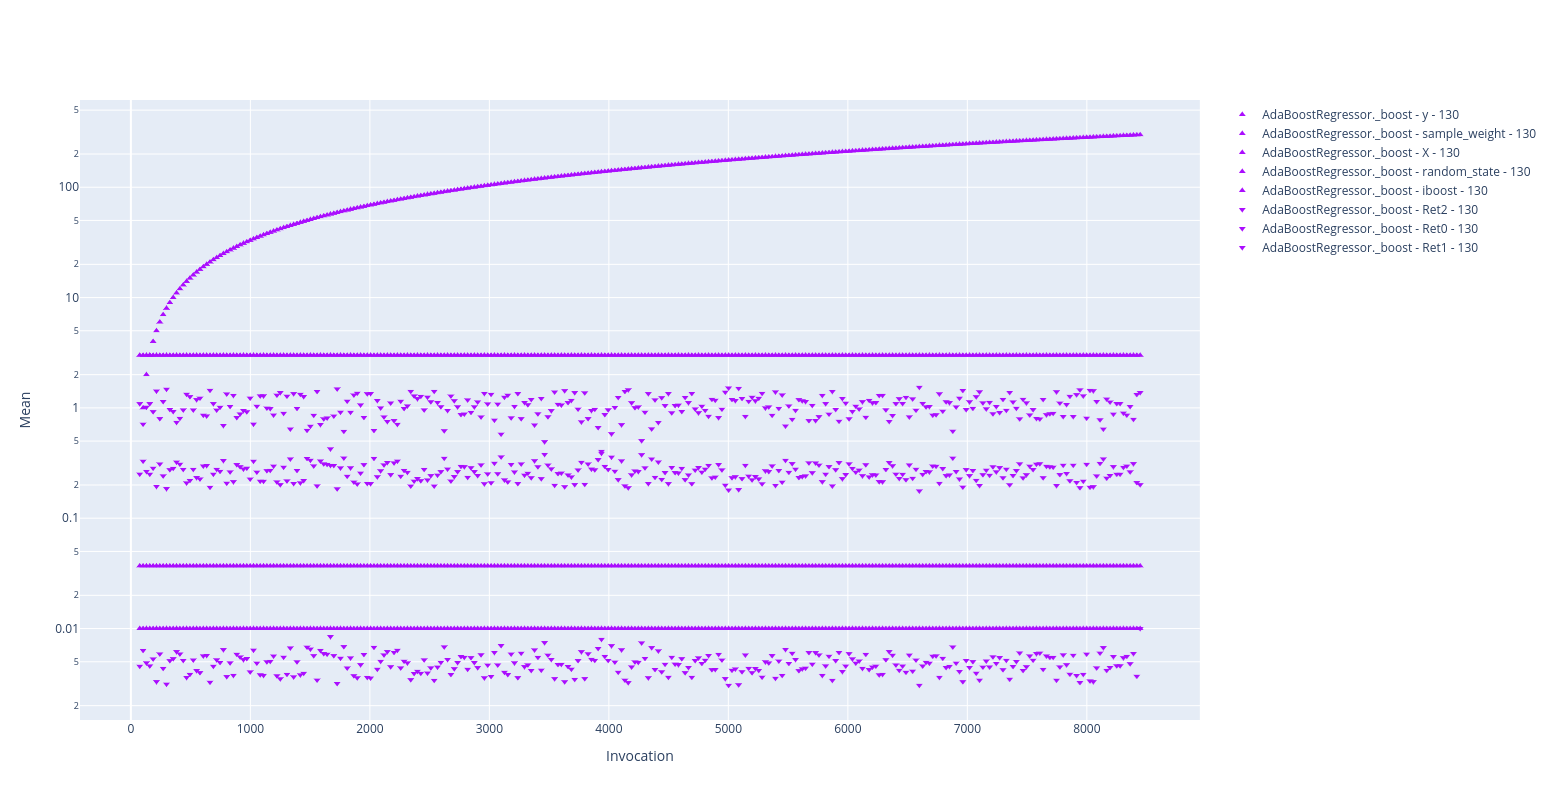
\includegraphics[width=\linewidth]{figure/adaboost/adaboost_boost_mean.png}
%     \caption{Mean values of boost function.}
%     \label{fig:adaboost_boost_mean}
% \end{figure}

% \begin{figure}
%     \centering
%     \caption{Caption}
%     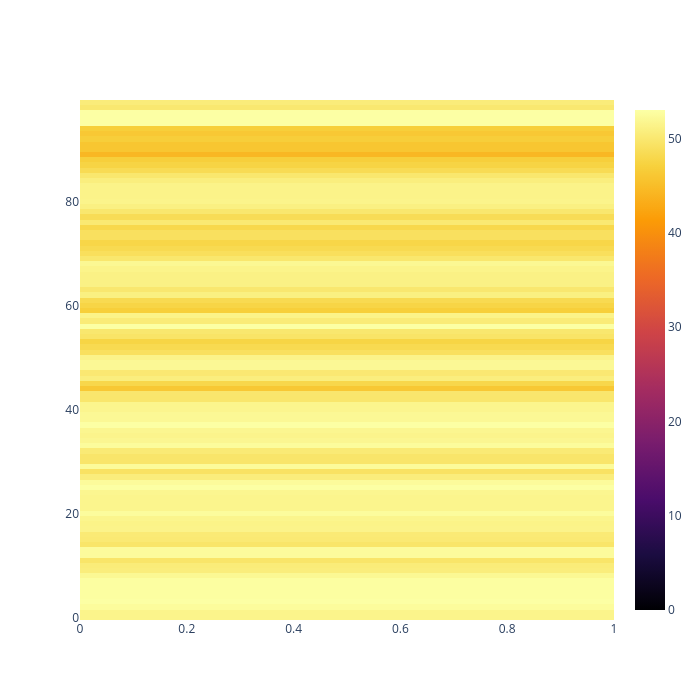
\includegraphics[width=\linewidth]{figure/adaboost/predict_adaboost_zoom_s.png}
%     \caption{Average number of significant digits of prediction over estimator}
%     \label{fig:adaboost_predict_zoom_s}
% \end{figure}

% \begin{figure}
% \begin{minipage}{0.4\linewidth}
%     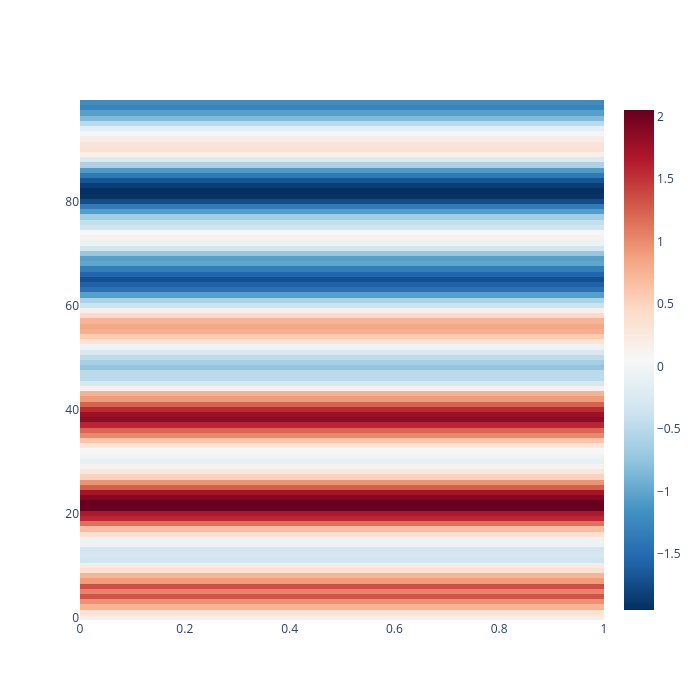
\includegraphics[width=\linewidth]{figure/adaboost/to_predict_adaboost_mean.png}
%     \caption{Values to predict}
%     \label{fig:adaboost_to_predict_mean}
% \end{minipage}
% \begin{minipage}{0.4\linewidth}
%     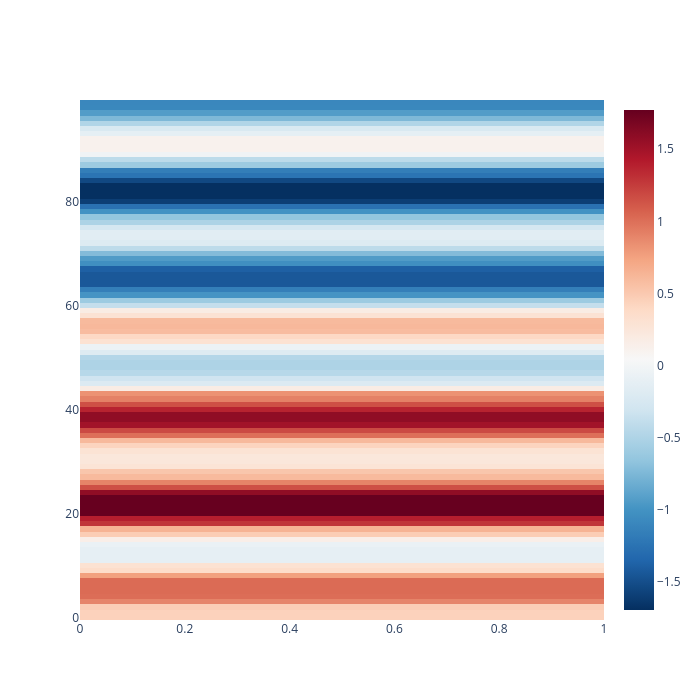
\includegraphics[width=\linewidth]{figure/adaboost/predict_adaboost_zoom_mean.png}
%     \caption{Predicted values}
%     \label{fig:adaboost_predicted_mean}
% \end{minipage}
% \caption{Comparison between original (fig.~\ref{fig:adaboost_to_predict_mean}) and predicted (fig.~\ref{fig:adaboost_predicted_mean}) values}
% \end{figure}

% \subsubsection{Bayesian Ridge Regression}

% "\texttt{BayesianRidge} estimates a probabilistic model of the regression problem as described above. 
% The prior for the coefficient  is given by a spherical Gaussian:
% \[
%     p(w|\lambda)=\mathcal{N}(w|0,\lambda^{-1}\mathbf{I}_p)
% \]
% The priors over  and  are chosen to be gamma distributions, the conjugate prior for the precision of the Gaussian. 
% The resulting model is called Bayesian Ridge Regression, and is similar to the classical Ridge.
% The parameters, and are estimated jointly during the fit of the model, 
% the regularization parameters and being estimated by maximizing the log marginal likelihood. 
% The scikit-learn implementation is based on the algorithm~\cite{tipping2001sparse}."

% Both execution with RR and MCA modes failed but two different errors. 
% Execution in RR mode raises an error due to an invalid value encountered in the \texttt{sqrt} function
% while the MCA mode execution raises an error due to an issue with the Singular Value Decomposition (SVD) divergence.

% RR executions fail with an invalid value in the \texttt{sqrt} function 
% used in the \texttt{\_update\_coef\_} method of the \texttt{BayesianRidge} class.
% This method updates the posterior mean and compute the corresponding Root-Mean-Square-Error (rmse).

% When we backtrack the error propagation, we see that 

% MCA executions show the limit of Pytracer since the SVD decomposition in scipy is a wrapper around the 
% \texttt{gesdd} or \texttt{gesvd} LAPACK~\cite{anderson1999lapack} functions. 
% Numerical instabilities that are coming from this kernel are opaque for Pytracer since it works 
% at the Python level. Tools working on C/FORTAN codes 
% like Veritracer~\cite{chatelain2018veritracer} can be used to zoom in on these functions.
% Nevertheless, Pytracer provides have a visualization of the input used by the SVD and several
% metrics used in numerical analysis, like the condition number, that can help to understand.

\subsubsection{Classifier comparisions}

This test compares the performance of 6 online solvers on the hand-written digits dataset.
These 6 solvers are:
\begin{itemize}
    \item Stochastic Gradient Descent 
    \item Averaged Stochastic Gradient Decent
    \item Perceptron
    \item Passive-Aggressive I \& II
    \item SAG: Minimizing Finite Sums with the Stochastic Average Gradient
\end{itemize}

Each solver is trained and predicts 20 times on 6 different training size ratio.
Figure~\ref{fig:classifier_comparisons_general} shows the all functions
traced by Pytracer over time. We can see the estimated number of significant digits varies a lot between 
values from 1 to 80 bits. Figure~\ref{fig:classifier_comparisons_mean_predictions} shows 
the average prediction score for each classifiers. The yellow points 
represent the average correct prediction score for one round and one classifier (line. 48) while blue points
tshows average predictions over the 20 rounds (line. 49).
We can see that precision is pretty low with an average solution below 10 significant bits, with 
an exception for values between the 24k and 32k invocation that correspond to the Perceptron
classifier. Indeed, this classifier is pretty stable with an average number of significant digits around 52 bits.

\begin{figure}
    \begin{lstlisting}[language=Python,style=customPython,numbers=left, firstnumber=19]
heldout = [0.95, 0.90, 0.75, 0.50, 0.01]
rounds = 20
X, y = datasets.load_digits(return_X_y=True)

classifiers = [
    ("SGD", SGDClassifier(max_iter=100)),
    ("ASGD", SGDClassifier(average=True)),
    ("Perceptron", Perceptron()),
    ("Passive-Aggressive I", PassiveAggressiveClassifier(loss='hinge',C=1.0, tol=1e-4)),
    ("Passive-Aggressive II", PassiveAggressiveClassifier(loss='squared_hinge',C=1.0, tol=1e-4)),
    ("SAG", LogisticRegression(solver='sag', tol=1e-1, C=1.e4 / X.shape[0]))
]

xx = 1. - np.array(heldout)

for name, clf in classifiers:
    print("training %s" % name)
    rng = np.random.RandomState(42)
    yy = []
    for i in heldout:
        yy_ = []
        for r in range(rounds):
            X_train, X_test, y_train, y_test = train_test_split(X, y, test_size=i, random_state=rng)
            clf.fit(X_train, y_train)
            y_pred = clf.predict(X_test)
            yy_.append(1 - np.mean(y_pred == y_test))
        yy.append(np.mean(yy_))
    plt.plot(xx, yy, label=name)
    \end{lstlisting}
    \label{fig:wrapper_code}
\caption{Illustration of the issue of using \texttt{frompyfunc} function to convert function to \texttt{ufunc}.}
\end{figure}

\begin{figure}
    \centering
    \caption{Caption}
    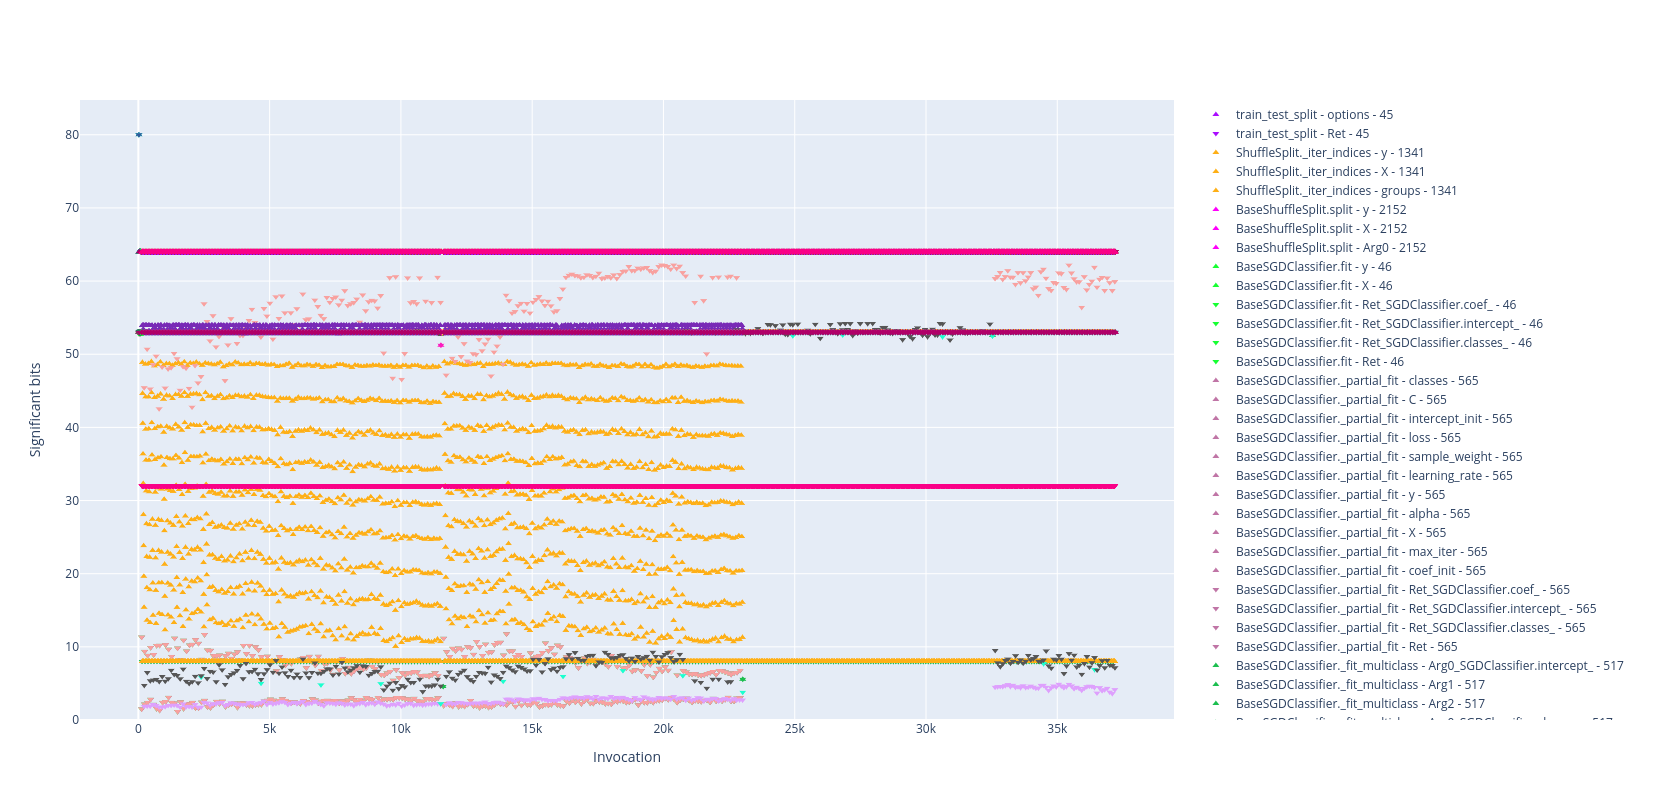
\includegraphics[width=\linewidth]{figure/classifier_comparisons/general.png}
    \caption{Number of significant digits (General view).}
    \label{fig:classifier_comparisons_general}
\end{figure}

\begin{figure}
    \centering
    \caption{Caption}
    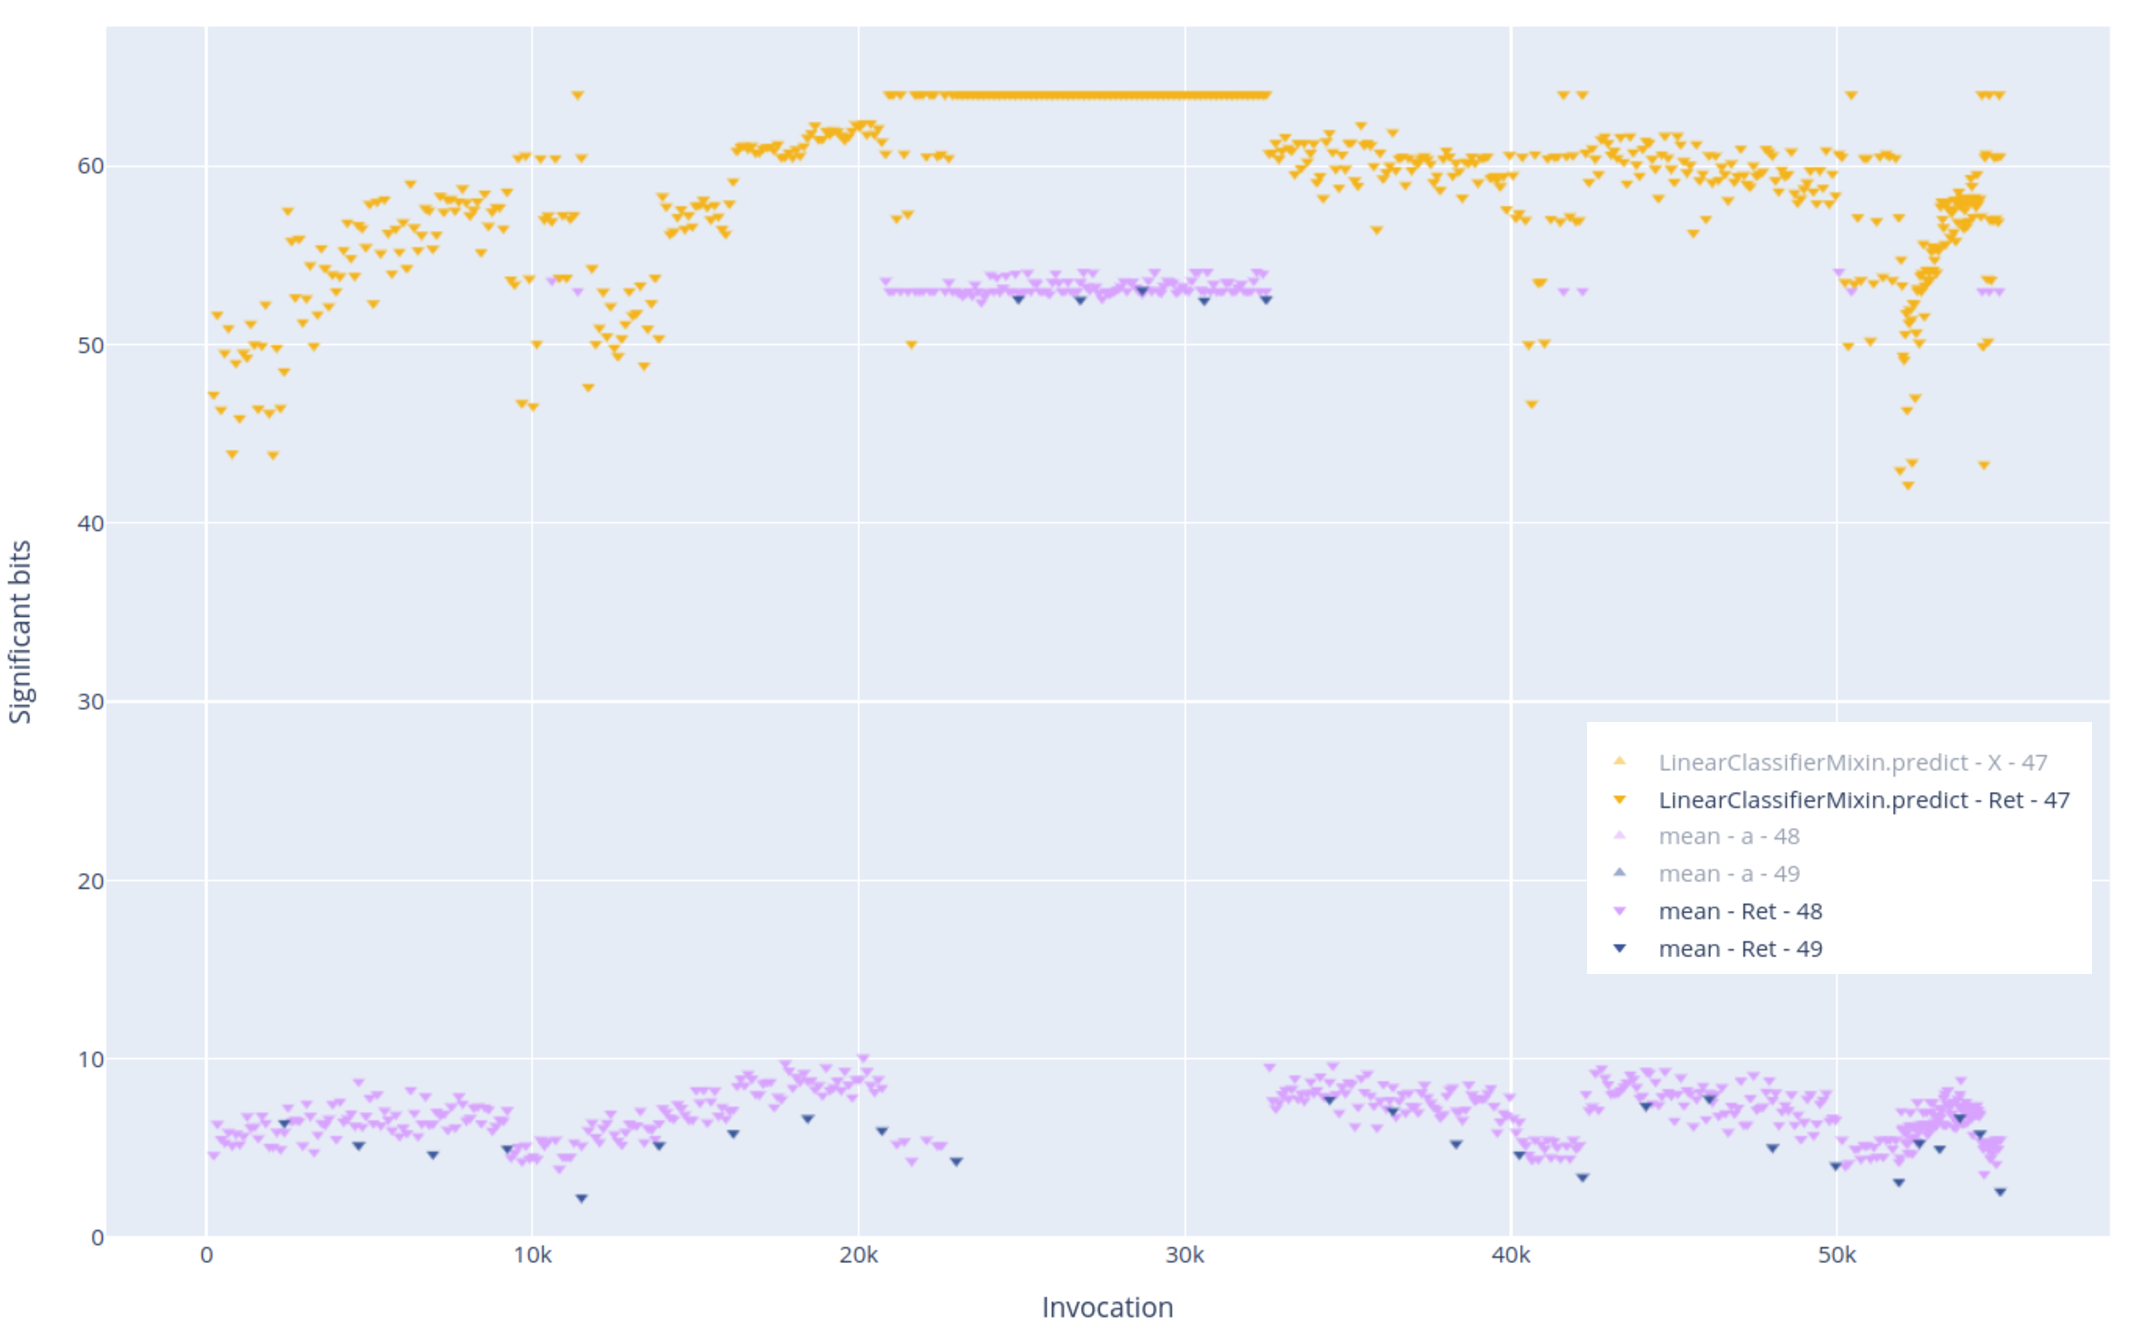
\includegraphics[width=\linewidth]{figure/classifier_comparisons/mean_prediction_wo_legend.pdf}
    \caption{Number of significant digits of the accuracy and predictions for the five classifiers. 
    Yellow points represents the accuracy for each round and blue points the average accuracy 
    over the 20 rounds. We can see that the Perceptron classifier has the highest stability.}
    \label{fig:classifier_comparisons_mean_predictions}
\end{figure}

% \begin{figure}
%     \centering
%     \caption{Caption}
%     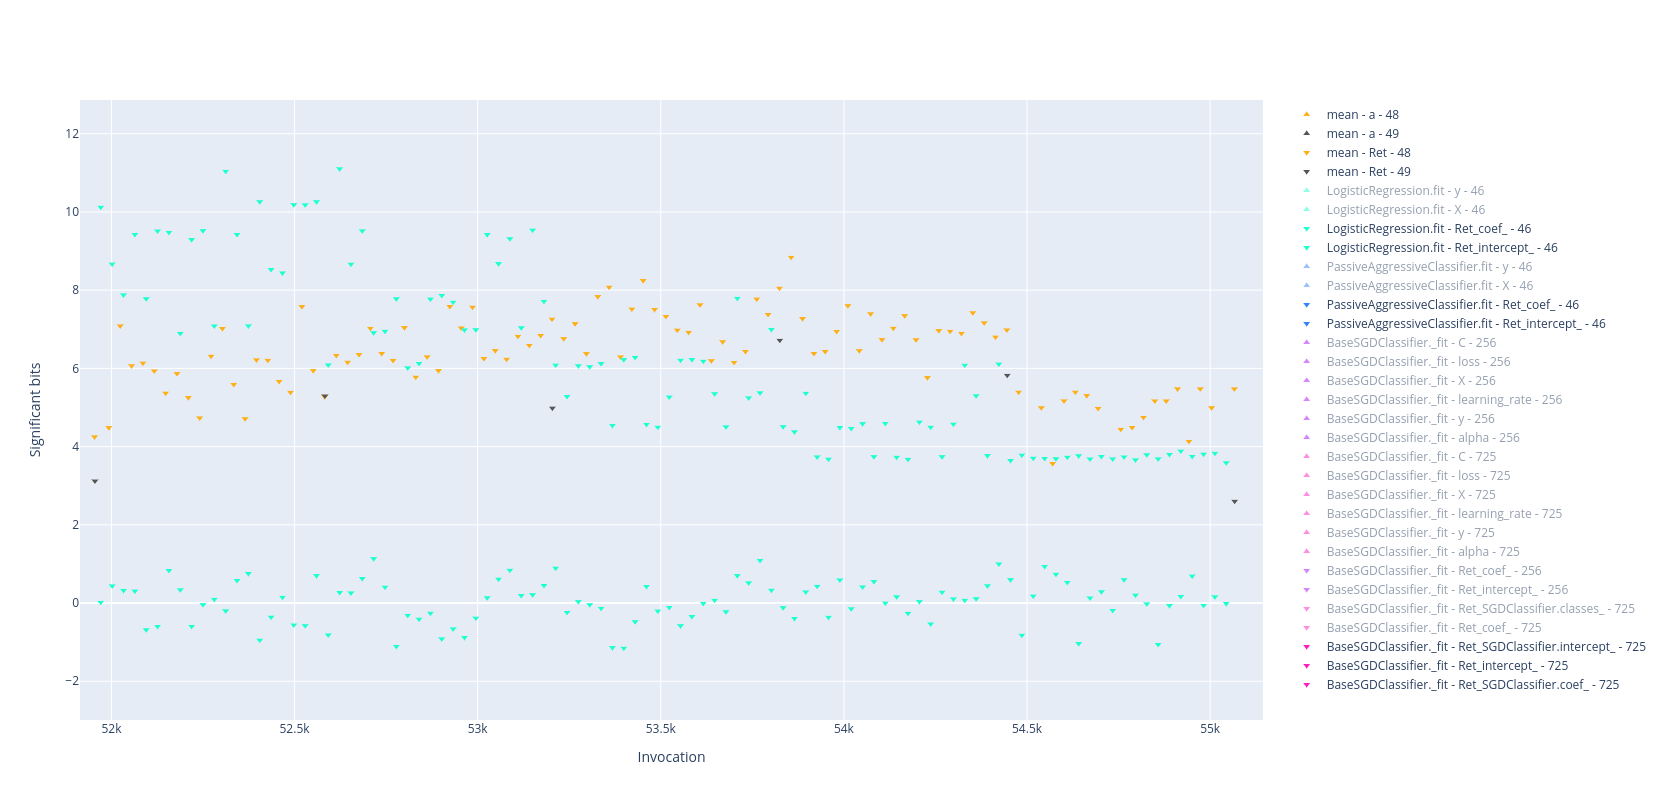
\includegraphics[width=\linewidth]{figure/classifier_comparisons/SAG_predicition_s.png}
%     \caption{Number of significant digits (General view).}
%     \label{fig:classifier_comparisons_general}
% \end{figure}

% \begin{figure}
%     \centering
%     \caption{Caption}
%     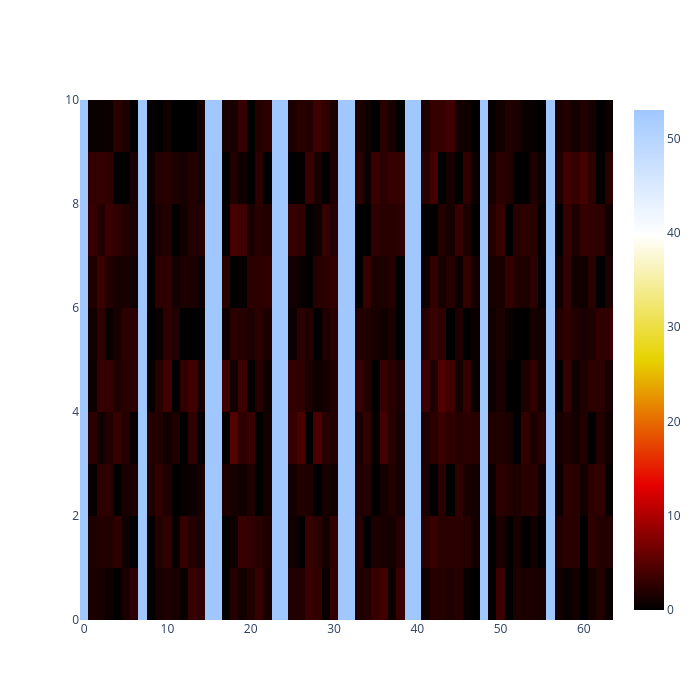
\includegraphics[width=\linewidth]{figure/classifier_comparisons/zoom_SAG_fit_coef_s.png}
%     \caption{Number of significant digits (General view).}
%     \label{fig:classifier_comparisons_general}
% \end{figure}


\subsubsection{Cluster IRIS}


\begin{figure}
    \centering
    \caption{Caption}
    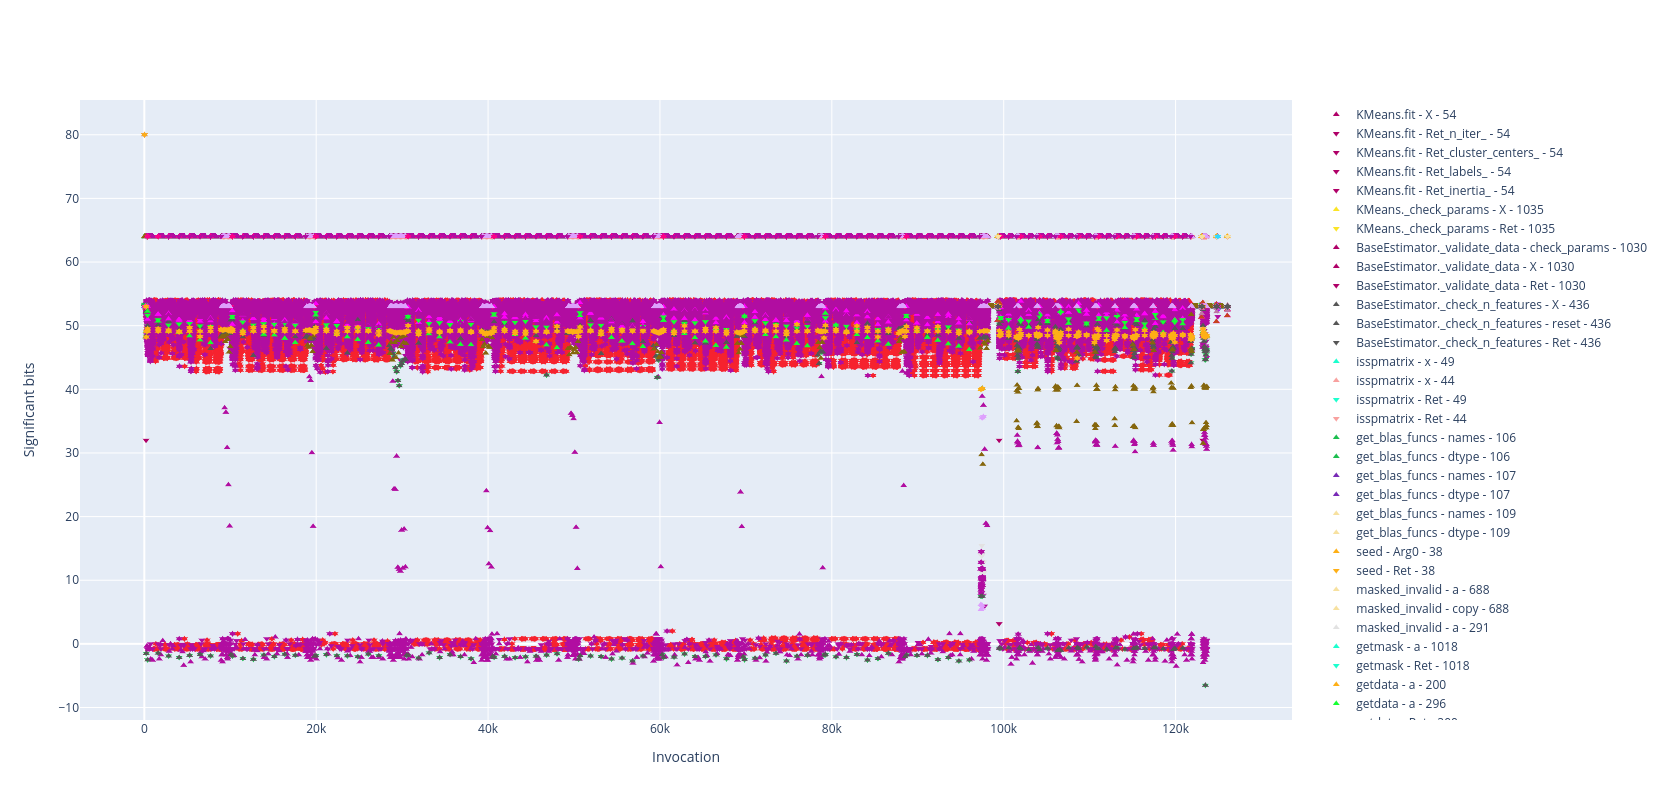
\includegraphics[width=\linewidth]{figure/cluster_iris/general.png}
    \caption{Number of significant digits of the Cluster IRIS test.}
    \label{fig:cluster_iris_general}
\end{figure}

\subsection{PyAFQ}


PyAFQ is Python package for Automated Fiber Quantification.
It aims at finding delineation of the major fiber tracts in individual human brains, and quantification of the tissue properties within the tracts.

\section{Performance evaluation}

In this section, we review the performance overhead of the Pytracer's instrumentation cost
and the time spent during the postprocessing analysis. 

\subsection{Overhead}

Pytracer instrumentation overhead comes from the time spent to instrument module (initial ?zation overhead)
before executing the targeted application plus the cost for dumping the data during the execution (running overhead).
However, initialization overhead is amortized when traced applications are above ....
Table~\ref{tab:pytracer_overhead} summaries the slowdown measure on pyAFQ test.
We can see that Pytracer only a gives reasonable slowdown of $\times 6$.

\begin{table}[]
    \centering
    \begin{tabular}{c|c|c|c|c}
         Pytracer & Verificarlo Instrumentation & Backend & Time (hours:minutes:seconds) & Overhead \\
         \hline 
         No & No & - & 00:30:51 & 1 \\
         No & Yes & IEEE & 01:32:56 & 3 \\
         No & Yes & RR & 16:52:08 & 32 \\
         Yes & No & - & 03:11:07 & 6  \\
         Yes & Yes & IEEE & 11:14:33 & 22 \\
         Yes & Yes & RR & 25:05:54 & 48 \\
    \end{tabular}
    \caption{Overheads of \pytracer on PyAFQ experiment with and without fuzzy.}
    \label{tab:pytracer_overhead}
\end{table}

% \begin{table}[]
%     \centering
%     \begin{tabular}{c|c|c|c|c}
%          Pytracer & Verificarlo Instrumentation & Backend & Time (hours:minutes:seconds) & Overhead \\
%          \hline 
%          No & No & - & 15 & 1 \\
%          No & Yes & IEEE & 49 & 3 \\
%          No & Yes & RR &  & 441 & 29 \\
%          Yes & No & - & 03:11:07 & 6  \\
%          Yes & Yes & IEEE & 11:14:33 & 22 \\
%          Yes & Yes & RR & 25:05:54 & 48 \\
%     \end{tabular}
%     \caption{Caption}
%     \label{tab:pytracer_overhead}
% \end{table}

\subsection{Postprocessing}

Pytracer produces traces during the tracing phase that must be aggregated before visualizing.
Each trace is read sequentially until the end of the file. 
For the moment, Pytracer is not able to merge traces but we would like to extend it.
We measure the postprocessing time depending on the regularity of the 
trace and the batchsize.

\section{Discussion}

\pytracer is a tool for visualizing the numerical quality of function inputs/outputs over time.
It generates numerical traces that are aggregated in postprocessing to measure numerical discrepancies between executions.
\pytracer does not make any assumption about the noise model used to estimate uncertainties but has been tested with the MCA 
through the fuzzy ecosystem on two broadly used scientific libraries for Python with a partial success.

As we shown in the section~\ref{sec:impact_mca_modes}, using the Full MCA mode leads to run-time errors
that has a considerable impact on the proper functioning of the execution. This is unfortunate since these
errors do not reflect real numerical errors but errors related to perturbations that should not occur.
Fixing this misbehaviour would greatly help in the use of Full MCA mode since this mode allows simulating catastrophic
cancellations which are common sources of numerical errors. By preserving exact operations, RR mode is far more conservative 
and can be used more easily even though it does not simulate all perturbations that might be encountered.

Also, by using a postprocess analysis to aggregate traces, \pytracer falls in the same pitfalls than veritracer
and is limited to aggregate traces where execution flow path extremely diverge. A posteriori reconstruction
is a challenging task as one must be able to identify precisely flow path taken and to find synchronization points
to pursue the analysis. We retrieve for example this divergence behaviour in two general classes of numerical schemes:
iterative methods and optimization processes. One solution to overcome this issue is to 
integrate method used in code coverage analysis to keep track of flow paths taken in addition to the backtraces.
But this would increase the complexity of the postprocess analysis as well as an extra slowdown factor.
However, we believe that by coupling the gantt chart with a static analysis, \pytracer would be able to catch 
some divergence patterns occurring within a function. Indeed, by instrumenting at the function level, \pytracer 
has a view on function's callees (i.e. the functions that are called within a function) and thus should be able to
partially detect flow divergences.

By design principle, \pytracer is flexible on the noise model used although we only test it with the MCA model in our experiments.
But we would like to compare different models against MCA in future works to see the resulting differences. 
In particular, although \pytracer only works 
on sequential application for the moment, it can be used to analyze parallel section internal to a function.
The only restriction being that the section does not call other functions traced by \pytracer, 
we would fall in the previous issue of divergence if it would not be the case.
Since \pytracer only care about inputs and outputs of a function, the order of internal operations are transparent for it
and thus should be able to handle those cases.

Finally, elementary arithmetic operations are not instrumented by \pytracer and it can be a barrier to deeper analysis.
However, we believe that an instrumentation at the function level present two advantages:
it first limits the size of the traces since only inputs and outputs of a function are dumped instead 
of a full report which, on one hand, decrease the overhead of the instrumentation and, on the other hand,
help the user to quickly identify instabilities. One of the pitfalls can be to overwhelm the user with too much information, 
which makes analysis more difficult. Nevertheless, the analysis at fine granularity can be interesting 
at a final step of the understanding. Such an analysis would require a different instrumentation approach
by for example working at the Abstract Syntax Tree (AST) level since it is trivial to get it in Python.
An ideal way to do that would be to be able to extract and replay a function,
in the same vein as the CERE~\cite{castro2015cere} tool does but for Python, and use an AST instrumentation to analyze step by step 
the numerical quality of elementary operations within the fuzzy environment.
Lastly, AST analysis can serve as a basis for finding relationship between variables which is another useful 
piece of information for the user.

\tristan{I moved this paragraph from results, it belongs here. It should be weaved in the discussion.}
In addition to runtime errors that it raises, mismatching shapes is also a problem when aggregating
traces as \pytracer will not be able to compute statistics for set of arrays having different shapes.
Two solutions exist to overcome this issue: the first one is to not instrument the \texttt{PyArray\_Arange}
function with MCA. The advantage is that it is easy to set up since it requires one extra line in the exclusion file.
However, the same kind of problem may appear somewhere else
because, as we have seen, the operations being evolved are elementary. The chances that developers reproduce
the same pattern is very probable. The second solution is to ensure that Full MCA mode preserved the exact operations.
This solution has the advantage of not having to worry about which functions should be instrumented or not with MCA,
but it is hard to achieve it in practice. Indeed, we rely on the MCA implementation provided by Verificarlo that 
uses an internal precision to add the random perturbation that is higher 
than the working precision for applying the random noise. The result is then rounded to the working precision before returning it so
any residual noise lower than the working precision is lost. 
Keeping track of that noise would requires to record each intermediate computation in a shadow memory 
or at least to keep a tag about their exactness.
\Yohan{This idea has emerged by discussing with the Verificarlo's team. 
I must find a way to express that, and to do not give the impression that we discovered or suggest it.}
This option would require more extra works than the first one but would ensure more consistent results.


\Yohan{Discuss issue to visualize complex values (fft2D)}

\section{Conclusion}

\tristan{I moved this from the opening of Section 4, as this reads more like a summary of \pytracer's features than an experiment description. It should be refactored in 1-2 paragraphs summarizing the main properties of \pytracer.}
Our strategy is to demonstrate that \pytracer is:
\begin{itemize}
    \item Domain agnostic: \pytracer is intended to work on any scientific Python applications, 
    without specific domain specific languages or needs to rely on specific libraries.
    We target two of the most common libraries used in scientific computing within Python, SciPy and Scikit-learn, as
    well as a domain specific application in neuroimaging. We show that \pytracer works
    well on these libraries, capturing most of the functions' module targeted.
    \item Automatic: \pytracer objective is to offer an automatic instrumentation for any Python applications,
    from small prototype to state-of-the-art scientific libraries. 
    \item Scalable: \pytracer goal is to trace real world application and use case.
    In that perspective, we use \pytracer on PyAFQ, a domain specific application in neuroimaging to compute 
    tractograms, generating \pytracer traces up to 1TB. We demonstrate that \pytracer is able to 
    handle this volume of data and to offer an interactive and fluent visualization to the user.
    We also show that \pytracer instrumentation gives a slowdown of $\times 6$.
    \item Fuzzy compatible: \pytracer aims at evaluating numerical stability by using injection noise model.
    Although the noise model used is orthogonal to \pytracer tracing mechanism, we emphasis in these experiments 
    on the MCA model through the fuzzy environment, and discuss its compatibility with \pytracer tracing mechanism
    to point out limitations of the trace-based approach and to propose research tracks to overcome them.
    It should be noted that experiments conducted in this paper are the first largest application of the fuzzy ecosystem
    by the wide range of applications covered. We therefore found interesting to give a feedback about pitfalls and benefits encountered
    in order to shed light on the good and bad practices for first-time users and hence democratize the usage of MCA.
    Moreover, these analyses will help the fuzzy developers to increase the overall stability of fuzzy.
\end{itemize}

\bibliographystyle{abbrv}
\bibliography{biblio}

%%
%% If your work has an appendix, this is the place to put it.
\appendix

\end{document}
\endinput
%%
%% End of file `sample-authordraft.tex'.
